\section{信号的分解}

这一章主要涉及傅里叶变换(Fourier transform)。假设我们有一个信号 $y = f(t)$,
我们希望能将其变成 $y' = F(\omega)$ 的形式。
我们可以考虑将 $f(t)$ 展开为
\begin{align*}
    f(t) = \sum_{n = -\infty}^{\infty} c_n\varphi_n(t)
\end{align*}
的形式,找出 $\varphi_n(t) = \mathe^{\mathi n\omega_i t}$ 中的常数 $w_i$。
这说明 $\varphi_n(t)$ 中含有关于 $w_i$ 的信息。
这样,统计 $f(t)$ 在频率域($\omega$)上的分布,我们就得到了 $F(\omega)$。

\subsection{信号的分解方法}

信号有多种方法可以进行分解:
\begin{itemize}
    \item 直流分量 + 交流分量
    \item 偶分量 + 奇分量
    \item 实部分量 + 虚部分量
    \item 脉冲分量
    \item 基于正交分量的分解
\end{itemize}

\begin{definition}[信号的直流/交流分解]
    设 $f(t)$ 为一个信号,定义其\bd{直流分量}为
    \begin{align*}
        f_{\text{AC}} = \lim_{T \to \infty}\frac{1}{T}\int_{T/2}^{-T/2}f(t)\D{t},
    \end{align*}
    其\bd{交流分量}为
    \begin{align*}
        f_{\text{AC}}(t) = f(t) - f_{\text{DC}}.
    \end{align*}
\end{definition}

\begin{definition}[信号的奇/偶分解]
    设 $f(t)$ 是一个信号,定义其\bd{奇分量}为
    \begin{align*}
        f_{\text{o}}(t) = \text{Od}[f(t)] = \frac{f(t) - f(-t)}{2},
    \end{align*}
    其\bd{偶分量}为
    \begin{align*}
        f_{\text{e}}(t) = \text{Ev}[f(t)] = \frac{f(t) + f(-t)}{2}.
    \end{align*}
\end{definition}

\begin{definition}[信号的实部/虚部分解]
    设 $f(t)$ 是一个信号,定义其\bd{实部分量}为
    \begin{align*}
        f_{\text{r}}(t) = \re[f(t)] = \frac{f(t) + f^*(t)}{2},
    \end{align*}
    其\bd{虚部分量}为
    \begin{align*}
        f_{\text{i}}(t) = \im[f(t)] = \frac{f(t) - f^*(t)}{2\mathi}.
    \end{align*}
\end{definition}

\begin{definition}[信号的脉冲分解]
    信号的\bd{脉冲分解}是指,信号可以近似地被表示为一组矩形脉冲的和的形式。
    设 $f(t)$ 是一个信号,定义其在 $t_1$ 处的矩形脉冲可以表示为如图 \ref{fig:rect-pulse-decomposition} 所示的函数:
    \begin{align*}
        f_{t_1}(t) = f(t_1)[u(t - t_1) - u(t - t_1 - \Delta t_1)],
    \end{align*}
    则 $f(t)$ 可以表示为
    \begin{align*}
        f(t) \approx \sum_{t_1 = -\infty}^{+\infty}f_{t_1}(t)
            = \sum_{t_1 = -\infty}^{+\infty}f(t_1)[u(t - t_1) - u(t - t_1 - \Delta t_1)].
    \end{align*}
    \begin{figure}[H]
        \centering
        \includegraphics[width=0.5\textwidth]{chap2/img/rect-pulse-decomposition}
        \caption{$f(t)$ 的脉冲分解}
        \label{fig:rect-pulse-decomposition}
    \end{figure}
\end{definition}

\begin{note}
    信号的直流/交流分解、奇/偶分解、实部/虚部分解的结果是\bd{唯一}的,脉冲分解是结果是\bd{近似}的。
\end{note}

\subsection{函数的正交分解}

\subsubsection{标准正交函数集}

\begin{definition}[平方可积函数]
    令 $x(t)$ 为一实函数,若
    \begin{align*}
        \int_{-\infty}^{+\infty}x^2(t)\D{t} < +\infty,
    \end{align*}
    则称 $x(t)$ 为\bd{平方可积函数},并记作 $x(t) \in L^2(\set{R})$。
    即,$L^2(\set{R})$ 表示所有平方可积函数组成的函数空间。
\end{definition}

\begin{definition}[内积]
    设 $f_1(t)$ 和 $f_2(t)$ 为两个函数,定义它们在区间 $[t_1, t_2]$ 上的\bd{内积}为
    \begin{align*}
        \ip{f_1}{f_2} = \int_{t_1}^{t_2}f_1(t)f_2^*(t)\D{t}.
    \end{align*}
\end{definition}

\begin{remark}
    回忆第 1 章中正交函数与正交函数集的定义,可以发现,$f_1(t)$ 和 $f_2(t)$ 在 $[t_1, t_2]$ 上正交,
    是指它们在 $[t_1, t_2]$ 上\bd{互不含有对方的分量}。函数 $f_1$ 和 $f_2$ 在 $[t_1, t_2]$ 上正交
    的充要条件是它们的内积为零。即,
    \begin{align*}
        \ip{f_1}{f_2} = 0.
    \end{align*}
\end{remark}

\begin{definition}[标准函数集]
    如果在区间 $[t_1, t_2]$ 上,函数集 $\{\varphi_i(t)\}$ 满足
    \begin{align*}
        \ip{\varphi_i}{\varphi_i} = \int_{t_1}^{t_2}\varphi_i(t)\varphi_i^*\D{t}
            = \int_{t_1}^{t_2}\|\varphi_i(t)\|^2\D{t} = 1,
    \end{align*}
    则称此函数集 $\{\varphi_i(t)\}$ 为\bd{标准函数集}。
\end{definition}

\begin{definition}[标准正交函数集]
    若正交函数集 $\{\varphi_i(t)\}$ 是一个标准函数集,则称之为\bd{标准正交函数集}。
\end{definition}

\subsubsection{函数的正交分解}

\begin{definition}[函数的正交分解]
    当函数 $f(t)$ 在 $[t_1, t_2]$ 区间具有连续的一阶导数和逐段连续的二阶导数时,
    $f(t)$ 可以用完备的正交函数集 $\{\varphi_i(t)\}$ 来表示,即
    \begin{align*}
        f(t) = \sum_{i = 1}^{+\infty}c_i\varphi_i(t),
    \end{align*}
    其中 $c_i$ 为常数,则称此表示为函数 $f(t)$ 的\bd{正交分解}。

    值得注意的事,$c_i$ 可以显式地表达为
    \begin{align*}
        c_i = \frac{\ip{f}{\varphi_i}}{\ip{\varphi_i}{\varphi_i}}
            = \frac{\ip{f}{\varphi_i}}{k_i}
            = \frac{1}{k_i}\int_{t_1}^{t_2}f(t)\varphi_i^*(t)\D{t},
    \end{align*}
    而 $k_i$ 为 $\varphi_i(t)$ 在区间 $[t_1, t_2]$ 上与自己的内积,即
    \begin{align*}
        k_i = \ip{\varphi_i}{\varphi_i} = \int_{t_1}^{t_2}\varphi_i(t)\varphi_i^*(t)\D{t}
        = \int_{t_1}^{t_2}\|\varphi_i(t)\|^2\D{t}.
    \end{align*}
\end{definition}

\begin{theorem}[帕斯瓦尔定理]
    用一个正交函数集来准确地表示一个信号时,这信号的能量等于相应的正交函数各分量的能量之和。
    即,设 $f(t)$ 为一个信号,将用正交函数集 $\{\varphi_i(t)\}$ 来表示,$c_i, k_i$ 定义如上,
    则有
    \begin{align*}
        \int_{t_1}^{t_2}\|f(t)\|^2\D{t} = \sum_{i = 1}^{+\infty}\|c_i\|^2k_i.
    \end{align*}
    这被称为\bd{帕斯瓦尔(Parseval)定理}。
\end{theorem}

\begin{proof}
    由于 $\{\varphi_i(t)\}$ 是一个正交函数集,故有
    \begin{align*}
        \ip{\varphi_i}{\varphi_j} = \begin{cases}
            1, & i = j, \\
            0, & i \neq j.
        \end{cases}
    \end{align*}
    而 $f(t)$ 的正交分解为 $f(t) = \sum_{i = 1}^{+\infty}c_i\varphi_i(t)$,故有
    \begin{align*}
        \int_{t_1}^{t_2}\|f(t)\|^2\D{t} & = \int_{t_1}^{t_2}\left\|\sum_{i = 1}^{+\infty}c_i\varphi_i(t)\right\|^2\D{t} \\
        & = \int_{t_1}^{t_2}\sum_{i = 1}^{+\infty}\|c_i\varphi_i(t)\|^2\D{t}
            + \sum_{i, j \ge 1, i \neq j}\|c_ic_j^*\ip{\varphi_i}{\varphi_j}\| \\
        & = \int_{t_1}^{t_2}\sum_{i = 1}^{+\infty}\|c_i\|^2\cdot \|\varphi_i(t)\|^2\D{t} + 0 \\
        & = \sum_{i = 1}^{+\infty}\|c_i\|^2k_i.
    \end{align*}
\end{proof}

\begin{note}
    在推导的过程中,对于内积运算,别忘了\bd{取共轭}。例如上述证明中的 $c_j^*$。
\end{note}

\subsection{信号的正交变换}

\subsubsection{信号的级数展开}

\begin{definition}[信号的级数展开]
    考虑使用一组函数 $\{\varphi_i(t)\}$,将信号 $x(t) \in L^2(\set{R})$ 展开成级数,即
    \begin{align*}
        x(t) = \sum_{i = -\infty}^{+\infty}c_i\varphi_i(t),
    \end{align*}
    这一形式称为信号 $x(t)$ 的\bd{级数展开}。

    通常,展开系数 $c_i$ 使用信号 $x(t)$ 的某种积分形式来确定。这一积分公式(即求展开系数的公式)
    称之为\bd{信号变换}。
\end{definition}

\subsubsection{函数的正交变换}

\begin{definition}[函数的正交变换]
    若信号级数展开的基函数 $\{\varphi_i(t)\}$ 为标准完备正交函数集,则积分变换
    \begin{align*}
        c_i = \int_{t_1}^{t_2}x(t)\varphi_i^*(t)\D{t}
    \end{align*}
    称为信号 $x(t)$ 的\bd{正交变换},亦称为 \bd{Karhunen-Loève 变换}。
\end{definition}

\begin{note}
    如果信号为符合狄义赫利(Dirichlet)条件的周期函数,则正交分解的系数 $c_i$ 的形式会很漂亮。
\end{note}

\subsection{特例:周期函数的傅里叶级数}

\begin{remark}
    周期信号通常可以被表示为
    \begin{align*}
        f(t) = \sum_{n = -\infty}^{\infty} f_0(t - nT),
    \end{align*}
    其中 $f_0(t)$ 是一个周期为 $T$ 的函数。
\end{remark}

\subsubsection{周期函数的正交分解}

\begin{definition}[狄义赫利条件]
    设有一信号 $f(t)$,若它满足以下条件:
    \begin{enumerate}[label=(\arabic*)]
        \item $f(t)$ 间断点的个数有限,
        \item $f(t)$ 极值点的个数有限,
        \item $f(t)$ 绝对积分数值有限,
    \end{enumerate}
    则称 $f(t)$ 满足\bd{狄义赫利条件}。
\end{definition}

\begin{theorem}
    满足狄义赫利条件的\bd{周期函数}
    都可以在一组\bd{完备的正交基函数}上展开成为\bd{无穷级数}。
\end{theorem}

\begin{definition}[傅里叶级数展开]
    如果完备的正交函数集是三角函数集或指数函数集,
    则周期函数展成的级数就是\bd{傅里叶级数}。
    相应的级数通常被称为\bd{三角形式傅里叶级数}和\bd{指数形式傅里叶级数}。
\end{definition}

\begin{note}
    回忆三角函数集和指数函数集的定义:
    \begin{itemize}
        \item 三角函数集(不完备):$\{1, \cos(\omega_0t + \varphi_1), \cos(2\omega_0t + \varphi_2), \cdots, \cos(n\omega_0 t + \varphi_n)\}$,
            即 $\{1, \cos(n\omega_0t), \sin(n\omega_0t)\}$,其中 $n$ 取遍 $\set{N}^{+}$。
        \item 三角函数集(完备):$\{1, \cos(n\omega_0 t), \sin(n\omega_0 t)\}$,其中 $n$ 取遍 $\set{N}^{+}$。
        \item 指数函数集:$\{\mathe^{\mathi n\omega_0t} \mid n \in \set{Z}\}$。
    \end{itemize}
    请注意,三角函数集中的 $n$ 是\bd{正整数},而指数函数集中的 $n$ 是\bd{整数}。
\end{note}

\begin{definition}[三角形式傅里叶级数]
    设周期函数 $f(t)$ 的周期为 $T_0$,令 $\omega_0 = 2\pi/T_0$,
    函数集 $\{1, \cos(n\omega_0 t), \sin(n\omega_0 t)\}$ 是一组完备的正交函数集,
    其中 $n$ 取遍 $\set{N}^{+}$。则 $f(t)$ 可以被展开成三角函数的无穷级数形式:
    \begin{align*}
        f(t) = a_0 + \sum_{n = 1}^{+\infty}(a_n\cos(n\omega_0 t) + b_n\sin(n\omega_0 t)),
    \end{align*}
    系数 $a_n$ 和 $b_n$ 统称为\bd{三角形式的傅里叶级数系数},简称为\bd{傅里叶系数}。
\end{definition}

\begin{lemma}
    设周期函数 $f(t)$ 的周期为 $T_0$,令 $\omega_0 = 2\pi/T_0$,
    函数集 $\{1, \cos(n_0\omega_0 t), \sin(n_0\omega_0 t)\}$ 是一组完备的正交函数集,
    其中 $n$ 取遍 $\set{N}^{+}$。则
    \begin{align*}
        \int_{t_0}^{t_0 + T_0}\cos(m\omega_0 t)\cos (n\omega_0 t)\D{t} & = \begin{cases}
            T_0 / 2, & m = n \neq 0, \\
            T_0, & m = n = 0, \\
            0, & m \neq n.
        \end{cases} \\
        \int_{t_0}^{t_0 + T_0}\sin(m\omega_0 t)\sin (n\omega_0 t)\D{t} & = \begin{cases}
            T_0 / 2, & m = n \neq 0, \\
            0, & \text{otherwise}.
        \end{cases} \\
        \int_{t_0}^{t_0 + T_0}\cos(m\omega_0 t)\sin (n\omega_0 t)\D{t} & = 0.
    \end{align*}
\end{lemma}

\begin{proof}
    首先证明 $\cos(m\omega_0 t)\cos(n\omega_0 t)$ 的积分:
    \begin{align*}
        \int_{t_0}^{t_0 + T_0}\cos(m\omega_0 t)\cos(n\omega_0 t)\D{t}
        & = \frac{1}{2}\int_{t_0}^{t_0 + T_0}\left(\cos((m + n)\omega_0 t) + \cos((m - n)\omega_0 t)\right)\D{t} \\
        & = \begin{cases}
            T_0 / 2, & m = n \neq 0, \\
            T_0, & m = n = 0, \\
            0, & m \neq n.
        \end{cases}
    \end{align*}
    然后证明 $\sin(m\omega_0 t)\sin(n\omega_0 t)$ 的积分:
    \begin{align*}
        \int_{t_0}^{t_0 + T_0}\sin(m\omega_0 t)\sin(n\omega_0 t)\D{t}
        & = \frac{1}{2}\int_{t_0}^{t_0 + T_0}\left(\cos((m - n)\omega_0 t) - \cos((m + n)\omega_0 t)\right)\D{t} \\
        & = \begin{cases}
            T_0 / 2, & m = n \neq 0, \\
            0, & \text{otherwise}.
        \end{cases}
    \end{align*}
    最后证明 $\cos(m\omega_0 t)\sin(n\omega_0 t)$ 的积分:
    \begin{align*}
        \int_{t_0}^{t_0 + T_0}\cos(m\omega_0 t)\sin(n\omega_0 t)\D{t}
        & = \frac{1}{2}\int_{t_0}^{t_0 + T_0}\left(\sin((m + n)\omega_0 t) - \sin((m - n)\omega_0 t)\right)\D{t} \\
        & = 0.
    \end{align*}
    命题得证。
\end{proof}

\begin{corollary}
    傅里叶系数 $a_n$ 和 $b_n$ 的表达式为:
    \begin{align*}
        a_0 & = \frac{1}{T_0}\int_{t_0}^{t_0 + T_0}f(t)\D{t}, \\
        a_n & = \frac{2}{T_0}\int_{t_0}^{t_0 + T_0}f(t)\cos(n\omega_0 t)\D{t}, \\
        b_n & = \frac{2}{T_0}\int_{t_0}^{t_0 + T_0}f(t)\sin(n\omega_0 t)\D{t}.
    \end{align*}
\end{corollary}

\begin{proof}
    已知 $f(t) = a_0 + \sum_{n = 1}^{+\infty}a_n\cos(n\omega_0 t) + b_n\sin(n\omega_0 t)$,则
    等式两边同时在 $[t_0, t_0 + T_0]$ 上积分,有
    \begin{align*}
        \int_{t_0}^{t_0 + T_0}f(t)\D{t} & = \int_{t_0}^{t_0 + T_0}a_0\D{t} + \sum_{n = 1}^{+\infty}\int_{t_0}^{t_0 + T_0}a_n\cos(n\omega_0 t)\D{t} + \sum_{n = 1}^{+\infty}\int_{t_0}^{t_0 + T_0}b_n\sin(n\omega_0 t)\D{t} \\
        & = \int_{t_0}^{t_0 + T_0}a_0\D{t} + \sum_{n = 1}^{+\infty}a_n\int_{t_0}^{t_0 + T_0}\cos(n\omega_0 t)\D{t} + \sum_{n = 1}^{+\infty}b_n\int_{t_0}^{t_0 + T_0}\sin(n\omega_0 t)\D{t} \\
        & = T_0 \cdot a_0 + \sum_{n = 1}^{+\infty}a_n\cdot 0 + \sum_{n = 1}^{+\infty}b_n\cdot 0 \\
        & = T_0 \cdot a_0.
    \end{align*}
    因此,有 $a_0 = \frac{1}{T_0}\int_{t_0}^{t_0 + T_0}f(t)\D{t}$。

    同理,在等式左右两侧乘上 $\cos(n \omega_0 t)$ 之后再在 $[t_0, t_0 + T_0]$ 上积分,
    可得 $a_n = \frac{2}{T_0}\int_{t_0}^{t_0 + T_0}f(t)\cos(n\omega_0 t)\D{t}$。
    在等式左右两侧乘上 $\sin(n \omega_0 t)$ 之后再在 $[t_0, t_0 + T_0]$ 上积分,
    可得可得 $b_n = \frac{2}{T_0}\int_{t_0}^{t_0 + T_0}f(t)\sin(n\omega_0 t)\D{t}$。
    命题得证。
\end{proof}

\begin{remark}
    常用的正交函数集的基本函数,除正弦型函数(含复指数函数)外,
    还有勒让德函数(Legendre function)、贝塞尔函数(Bessel function)、
    沃尔什函数(Walsh function)等,不一一列举。
\end{remark}

\begin{definition}[复指数形式傅里叶级数]
    由欧拉公式可以得到 $\cos(n\omega_0 t) = (\mathe^{\mathi n\omega_0 t} + \mathe^{-\mathi n\omega_0 t}) / 2$,
    以及 $\sin(n\omega_0 t) = (\mathe^{\mathi n\omega_0 t} - \mathe^{-\mathi n\omega_0 t}) / 2\mathi$。
    因此,我们可以将三角函数形式的傅里叶级数改写为:
    \begin{align*}
        f(t) = a_0 + \sum_{i = 1}^{+\infty}\left(\frac{a_n - \mathi b_n}{2}\mathe^{\mathi n\omega_0 t} + \frac{a_n + \mathi b_n}{2}\mathe^{-\mathi n\omega_0 t}\right).
    \end{align*}
    记 $F(\cdot)$ 为一个函数,则 $a_0, a_n, b_n$ 可以看做是 $(n, \omega_0)$ 对应的函数值。则
    \begin{align*}
        f(t) = F(0) + \sum_{i = 1}^{+\infty}\left(F(n\omega_0)+ F(-n\omega_0)\right)
    \end{align*}
    再记 $F_n = F(n\omega_0)$,则可将 $f(t)$ 表示为\bd{复指数形式的傅里叶级数}:
    \begin{align*}
        f(t) = \sum_{n = -\infty}^{+\infty}F_n\mathe^{\mathi n\omega_0 t},
    \end{align*}
    其中 $F_n = (a_n - \mathi b_n) / 2$ 为\bd{复指数形式的傅里叶级数系数}。
\end{definition}

\begin{property}
    复指数形式傅里叶级数的系数 $F_n$ 的表达式为:
    \begin{align*}
        F_n = \frac{1}{T_0}\int_{t_0}^{t_0 + T_0}f(t)\mathe^{-\mathi n\omega_0 t}\D{t}.
    \end{align*}
\end{property}

\begin{proof}
    (方法一)
    \begin{align*}
        F_n & = \frac{a_n - \mathi b_n}{2} \\
        & = \frac{1}{2} \cdot \frac{2}{T_0}\int_{t_0}^{t_0 + T_0}f(t)\cos(n\omega_0 t)\D{t} - \frac{\mathi}{2} \cdot \frac{2}{T_0}\int_{t_0}^{t_0 + T_0}f(t)\sin(n\omega_0 t)\D{t} \\
        & = \frac{1}{T_0}\int_{t_0}^{t_0 + T_0}f(t)(\cos(n\omega_0 t) - \mathi \sin(n\omega_0 t))\D{t} \\
        & = \frac{1}{T_0}\int_{t_0}^{t_0 + T_0}f(t)\mathe^{-\mathi n\omega_0 t}\D{t}.
    \end{align*}
    命题得证。
\end{proof}

\begin{proof}
    (方法二)
    由级数展开的定义,在函数集 $\{\mathe^{\mathi n\omega_0 t}\}$ 上展开,有
    \begin{align*}
        F_n & = \frac{\ip{f}{\varphi_n}}{\ip{\varphi_n}{\varphi_n}}\\
        & = \frac{1}{k_n}\int_{t_0}^{t_0 + T_0}f(t) \mathe^{-\mathi n\omega_0 t}\D{t}.
    \end{align*}
    而 $k_n$ 可以计算如下:
    \begin{align*}
        k_n & = \int_{t_0}^{t_0 + T_0}\mathe^{\mathi n\omega_0 t}\mathe^{-\mathi n\omega_0 t}\D{t} \\
        & = \int_{t_0}^{t_0 + T_0}\D{t} \\
        & = T_0.
    \end{align*}
    因此 $F_n = \frac{1}{T_0}\int_{t_0}^{t_0 + T_0}f(t)\mathe^{-\mathi n\omega_0 t}\D{t}$。
\end{proof}

\begin{property}
    对偶信号序列的傅里叶级数而言,$F_n$ 是偶对称的实数序列,
    对奇信号序列的傅里叶级数而言,$F_n$ 是奇对称的纯虚序列。
\end{property}

\begin{proof}
    考虑关系式 $F_n = (a_n - \mathi b_n) / 2$:
    \begin{itemize}
        \item 对于偶信号序列而言,$a_n \neq 0, b_n = 0$,所以 $F_n$ 只有直流分量和余弦项。
        \item 对于奇信号序列而言,$a_n = 0, b_n \neq 0$,所以 $F_n$ 只有正弦项。
    \end{itemize}
    命题得证。
\end{proof}

\begin{corollary}[帕斯瓦尔定理的推论]
    周期信号的\bd{平均功率}等于傅里叶级数展开各谐波分量有效值的平方和。
    也就是说,\bd{时域和频域的能量守恒}。
\end{corollary}

\begin{proof}
    由帕斯瓦尔定理知,
    \begin{align*}
        \int_{t_0}^{t_0 + T_0}\|f(t)\|^2\D{t} & = \|a_0\|^2\cdot k_0
            + \sum_{i = 1}^{+\infty}\|a_i\|^2k_{\cos, i}
            + \sum_{i = 1}^{+\infty}\|b_i\|^2k_{\sin, i} \\
        & = T_0 \cdot \|a_0\|^2 + \frac{T_0}{2}\cdot \sum_{i = 1}^{+\infty}(\|a_i\|^2 + \|b_i\|^2).
    \end{align*}
    因此,有
    \begin{align*}
        P & = \overline{\|f(t)\|^2} = \frac{1}{T_0}\int_{t_0}^{t_0 + T_0}\|f(t)\|^2\D{t} \\
        & = \frac{1}{T_0}\left(T_0 \cdot \|a_0\|^2 + \frac{T_0}{2}\cdot \sum_{i = 1}^{+\infty}(\|a_i\|^2 + \|b_i\|^2)\right) \\
        & = \|a_0\|^2 + \frac{1}{2}\sum_{i = 1}^{+\infty}(\|a_i\|^2 + \|b_i\|^2) \\
        & = \sum_{i = -\infty}^{+\infty}\|F_n\|^2.
    \end{align*}
    命题得证。
\end{proof}

\subsubsection{周期信号的傅里叶级数}

\begin{definition}
    由于 $F_n \in \set{C}$,所以它谱线并不方便在二维平面上表示,
    因此 $F_n$ 可以从两个角度来表示:一个是 $|F_n|$,即为\bd{幅度谱},
    另一个是 $\varphi_n = \arg(F_n)$,即为\bd{相位谱}。

    周期信号的傅里叶级数可视化如图 \ref{fig:periodic-signal-fourier-series} 所示。
    \begin{figure}[H]
        \centering
        \includegraphics[width = 0.6\textwidth]{chap2/img/periodic-signal-fourier-series.png}
        \caption{周期信号的傅里叶级数}
        \label{fig:periodic-signal-fourier-series}
    \end{figure}
\end{definition}

\begin{property}[周期信号的傅里叶频谱特点]
    周期信号的傅里叶频谱有以下特点:
    \begin{itemize}
        \item 仅在一些离散的频率点 $n\omega_0, n \in \set{Z}$ 上有值。
        \item 离散间隔为 $\omega_0 = 2\pi f_0 = 2\pi / T_0$。
        \item $F_n$ 是双边谱,即 $F_n = F_{-n}$,因此正负频率的频谱幅度相加才是实际幅度。
        \item 信号的功率为 $\sum_{-\infty}^{+\infty}\|F_n\|^2$。
    \end{itemize}
\end{property}

\begin{example}[周期矩形脉冲信号的傅里叶级数]
    设周期矩形脉冲信号 $f(t)$ 的脉冲宽度为 $\tau$,脉冲幅度为 $E$,重复周期为 $T_0$。
    图像如图 \ref{fig:periodic-rect-pulse-signal} 所示。
    \begin{figure}[H]
        \centering
        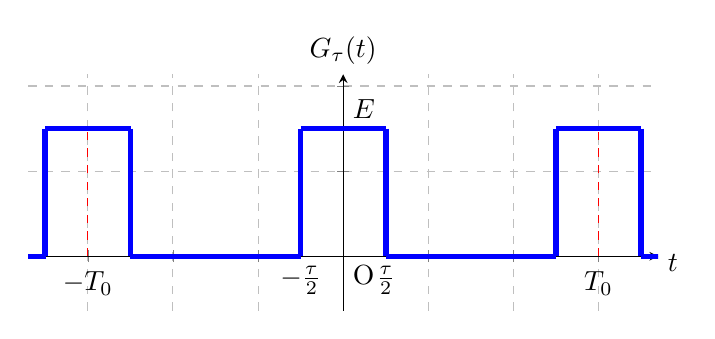
\begin{tikzpicture}
            \begin{axis}[
                axis lines = middle,
                xlabel = {$t$},
                xlabel style={at={(rel axis cs:1, 0.2)}, anchor=west},
                ylabel = {$G_{\tau}(t)$},
                ylabel style={at={(rel axis cs:0.5, 1)}, anchor=south},
                xmin = -3.7, xmax = 3.7,
                ymin = -0.2, ymax = 1.7,
                grid = major,
                grid style = dashed,
                scale only axis,
                width = 8cm,
                height = 3cm,
                axis equal,
                xtick = {-3, -2, -1, 0, 1, 2, 3},
                xticklabels = {$-T_0$, $ $, $ $, $ $, $ $, $ $, $T_0$},
                ytick = {0, 1, 2},
                yticklabels = {$ $, $ $, $ $},
            ]
            \addplot[domain=-3.7:-3.5, samples=100, smooth, line width=2pt, blue] {0};
            \addplot[smooth, line width=2pt, blue] coordinates {(-3.5, 0) (-3.5, 1.5)};
            \addplot[dashed, red] coordinates {(-3, 0) (-3, 1.5)};
            \addplot[domain=-3.5:-2.5, samples=100, smooth, line width=2pt, blue] {1.5};
            \addplot[smooth, line width=2pt, blue] coordinates {(-2.5, 1.5) (-2.5, 0)};
            \addplot[domain=-2.5:-0.5, samples=100, smooth, line width=2pt, blue] {0};
            \addplot[smooth, line width=2pt, blue] coordinates {(-0.5, 0) (-0.5, 1.5)};
            \addplot[domain=-0.5:0.5, samples=100, smooth, line width=2pt, blue] {1.5};
            \addplot[smooth, line width=2pt, blue] coordinates {(0.5, 1.5) (0.5, 0)};
            \addplot[domain=0.5:2.5, samples=100, smooth, line width=2pt, blue] {0};
            \addplot[smooth, line width=2pt, blue] coordinates {(2.5, 0) (2.5, 1.5)};
            \addplot[domain=2.5:3.5, samples=100, smooth, line width=2pt, blue] {1.5};
            \addplot[dashed, red] coordinates {(3, 0) (3, 1.5)};
            \addplot[smooth, line width=2pt, blue] coordinates {(3.5, 1.5) (3.5, 0)};
            \addplot[domain=3.5:3.7, samples=100, smooth, line width=2pt, blue] {0};
            \node at (axis cs:0, 0) [anchor=north west] {O};
            \node at (axis cs:0, 1.5) [anchor=south west] {$E$};
            \node at (axis cs:-0.5, 0) [anchor = north] {$-\frac{\tau}{2}$};
            \node at (axis cs:0.5, 0) [anchor = north] {$\frac{\tau}{2}$};
            \end{axis}
        \end{tikzpicture}
        \caption{周期矩形脉冲信号}
        \label{fig:periodic-rect-pulse-signal}
    \end{figure}

    则其在频域上的图像如图 \ref{fig:periodic-rect-pulse-signal-freq} 所示。
    \begin{figure}[H]
        \centering
        \begin{tikzpicture}
            \begin{axis}[
                axis lines = middle,
                xlabel = {$\omega$},
                ylabel = {$F_n$},
                ylabel style={at={(rel axis cs:0.5, 1)}, anchor=south},
                xmin = -10, xmax = 10,
                ymin = -0.3, ymax = 1.1,
                xtick = {-10, -8, -6, -4, -2, 0, 2, 4, 6, 8, 10},
                xticklabels = {$ $, $ $, $ $, $ $, $ $, $ $, $ $, $ $, $ $, $ $, $ $},
                ytick distance = 0.25,
                ytick = {-0.25, 0, 0.25, 0.5, 0.75, 1},
                yticklabels = {$ $, $ $, $ $, $ $, $ $, $\dfrac{E\tau}{T_0}$},
                grid = major,
                grid style = dashed,
            ]
            \addplot[dashed, domain=-10:10, samples=100, smooth, line width=2pt, blue] {sin(deg(x))/x};
            \draw[-stealth, smooth, line width=1pt, red] (axis cs:-8.3776, 0) -- (axis cs:-8.3776, 0.1034);
            \draw[-stealth, smooth, line width=1pt, red] (axis cs:-4.1888, 0) -- (axis cs:-4.1888, -0.2067);
            \draw[-stealth, smooth, line width=1pt, red] (axis cs:0, 0) -- (axis cs:0, 1);
            \draw[-stealth, smooth, line width=1pt, red] (axis cs:4.1888, 0) -- (axis cs:4.1888, -0.2067);
            \draw[-stealth, smooth, line width=1pt, red] (axis cs:8.3776, 0) -- (axis cs:8.3776, 0.1034);
            
            \node at (axis cs:0, 0) [anchor=north west] {O};
            \node at (axis cs:3.1416, 0) [anchor=north] {$\dfrac{2\pi}{\tau}$};
            \node at (axis cs:6.2832, 0) [anchor=north] {$\dfrac{4\pi}{\tau}$};
            \end{axis}
        \end{tikzpicture}
        \caption{周期矩形脉冲信号的频谱}
        \label{fig:periodic-rect-pulse-signal-freq}
    \end{figure}

    \begin{itemize}
        \item 谱线包络线为 $\sa$ 函数。
        \item 频谱谱线的间隔为 $\omega_0 = 2\pi / T_0$。
        \item 谱线包络线过零点位置为 $\omega_k = 2k\pi / \tau$,其中 $k \neq 0, k \in \set{Z}$。
    \end{itemize}
\end{example}

\begin{note}
    这里一般不考虑 $\omega_{-k}, k > 0$ 的情况。
\end{note}

\begin{theorem}
    周期为 $T_0$,脉冲宽度为 $\tau$,脉冲幅度为 $E$ 的周期矩形脉冲信号,谱线包络线则为
    \begin{align*}
        \frac{E\tau}{T_0}\sa{\left(\frac{\omega_0\tau}{2}\right)}.
    \end{align*}
\end{theorem}

\begin{proof}
    \begin{align*}
        F_n & = \frac{1}{T_0}\int_{-\tau/2}^{\tau/2}E\cdot \mathe^{-\mathi n\omega_0 t}\D{t} \\
        & = \frac{E}{T_0}\int_{-\tau/2}^{\tau/2}\mathe^{-\mathi n\omega_0 t}\D{t} \\
        & = \left.\frac{E}{T_0}\cdot\frac{1}{-\mathi n\omega_0}\cdot\left(\mathe^{-\mathi n\omega_0 t}\right)\right|_{-\tau/2}^{\tau/2} \\
        & = \frac{E}{T_0}\cdot\frac{1}{-\mathi n\omega_0}\cdot\left(\mathe^{-\mathi n\omega_0 \tau / 2} - \mathe^{\mathi n \omega_0\tau /2 }\right) \\
        & = \frac{E}{T_0}\cdot\frac{1}{-\mathi n\omega_0}\cdot\left(-2\mathi\sin\left(\frac{n\omega_0\tau}{2}\right)\right) \\
        & = \frac{E\tau}{T_0}\frac{\sin(n\omega_0\tau/2)}{n\omega_0\tau/2} \\
        & = \frac{E\tau}{T_0}\sa{\left(\frac{n\omega_0\tau}{2}\right)}.
    \end{align*}
\end{proof}

\begin{remark}
    非周期信号,在频率域上则为连续频谱;周期信号,在频率域上则为离散频谱。
    它们之间的转换关系,可以由下图 \ref{fig:periodic-nonperiodic-signal} 描述。
    \begin{figure}[H]
        \centering
        \includegraphics[width = 0.8\textwidth]{chap2/img/periodic-nonperiodic-signal.png}
        \caption{周期信号与非周期信号的频谱}
        \label{fig:periodic-nonperiodic-signal}
    \end{figure}
\end{remark}

\begin{property}[周期矩形脉冲信号的特点]
    在频域,能量主要集中在第一个零点以内!

    实际上,在允许一定失真的条件下,可以要求一个通信系统
    只把 $|\omega| \le 2\pi/\tau$ 频率范围内的各个频率分量传送过去,
    而舍弃 $|\omega| \ge 2\pi/\tau$ 的分量。

    常把 $-2\pi/\tau \le \omega \le 2\pi/\tau$ 这段频率范围成为矩形信号的\bd{频带宽度},
    简称\bd{带宽}。
    带宽只和脉冲的脉宽有关,而与脉高和周期均无关。
\end{property}

\begin{property}[周期信号的频谱谱线的特点]
    周期信号的频谱谱线的\bd{间隔}为
    \begin{align*}
        \omega_0 = \frac{2\pi}{T_0}.
    \end{align*}
    
    周期信号的频谱谱线的\bd{长度}为 $|F_n|$,其中
    \begin{align*}
        F_n = F(n\omega_0) = \frac{1}{T_0}\int_{t_0}^{t_0 + T_0}f(t)\mathe^{-\mathi n\omega_0 t}\D{t}.
    \end{align*}
\end{property}

\begin{note}
    由于复指数完备正交函数集中含有\bd{正负项},故周期矩形脉冲信号的谱线为\bd{双边谱}。
    对于 $n\omega_0$ 这一频率的频谱而言,频谱幅度为
    \begin{align*}
        |F_n| + |F_{-n}| = 2|F_n| = \frac{1}{2}\left(a_n^2 + b_n^2\right).
    \end{align*}
    一定要注意,它并不是 $|F_n|$。
\end{note}

\begin{homework}
    已知 $f(t) = \sin t\cos 2t + 5\cos 3t \sin 4t$,求该函数的傅里叶级数。
\end{homework}

\begin{solution}
    由三角函数的和差化积公式,有
    \begin{align*}
        f(t) & = \frac{1}{2}\left(\sin 3t - \sin t\right) + \frac{5}{2}\left(\sin 7t + \sin t\right) \\
        & = 2\sin t + \frac{1}{2}\sin 3t + \frac{5}{2}\sin 7t.
    \end{align*}
    此即为该函数的傅里叶级数。
\end{solution}

\subsection{非周期信号的傅里叶变换}

\subsubsection{非周期信号的傅里叶级数}

我们已经掌握了周期信号的傅里叶展开,那么如何处理非周期信号的傅里叶展开呢?
非周期信号可以看成是\bd{周期 $T_0$ 趋于无限大的周期信号},因此我们可以将非周期信号的傅里叶展开看成是周期信号的极限情况。

\begin{property}[非周期信号频谱性质]
    非周期信号的谱线间隔趋于 $0$,变成了\bd{连续频谱},谱线长度趋于 $0$。
\end{property}

\begin{proof}
    当 $T_0 \to +\infty$ 时,$\omega_0 = 2\pi / T_0 \to 0$,谱线间距变密直至为 $0$。$\omega$ 变为连续域。
    此时
    \begin{align*}
        F_n = \frac{1}{T_0}\int_{t_0}^{t_0 + T_0}f(t)\mathe^{-\mathi n\omega_0 t} \D{t} \to 0,
    \end{align*}
    谱线高度变矮直至为 $0$。
\end{proof}

\begin{remark}
    从物理意义着手:既然是信号,那么它必定会有能量;无论怎样,能量一定是守恒的。
    因此,频率域一定会以某种形式存在。

    从数学角度思考:无限多无穷小量的和,在极限意义下,可能等于一个有限值。
    谱线高度变矮直至为 $0$,只是说每个分量变成了无穷小量,但没有说总和(信号)为 $0$。
\end{remark}

\subsubsection{非周期信号的傅里叶变换}

有没有更优的非周期信号傅里叶频谱的定义方式?有,那就是\bd{傅里叶变换}。

\begin{definition}[非周期信号的傅里叶变换]
    设 $f(t)$ 是一个非周期信号,其傅里叶变换定义为
    \begin{equation}
        F(\omega) = \mathcal{F}[f(t)] = \int_{-\infty}^{+\infty}f(t)\mathe^{-\mathi\omega t} \D{t}.
    \end{equation}
    反之,想要恢复时域信号,$f(t)$ 可以通过逆变换得到:
    \begin{equation}
        f(t) = \mathcal{F}^{-1}[F(\omega)] = \frac{1}{2\pi}\int_{-\infty}^{+\infty}F(\omega)\mathe^{\mathi\omega t} \D{\omega}.
    \end{equation}
    这里的 $\mathcal{F}$ 和 $\mathcal{F}^{-1}$ 分别称为\bd{傅里叶变换}和\bd{傅里叶逆变换}。
\end{definition}

\begin{remark}
    傅里叶变换存在的充分条件:时域信号 $f(t)$ 绝对可积。
\end{remark}

\begin{definition}[傅里叶频谱]
    信号的傅里叶变换一般为复值函数,写成
    \begin{equation}
        F(\omega) = |F(\omega)|\mathe^{\mathi\phi(\omega)}.
    \end{equation}
    其中,$|F(\omega)|$ 称为\bd{幅度频谱密度函数},$\phi(\omega)$ 称为\bd{相位频谱密度函数}。
\end{definition}

\begin{example}
    设 $F(\omega) = \int_{-\infty}^{+\infty}f(t)\mathe^{-\mathi \omega t}\D{t} = R(\omega) + \mathi X(\omega)$,
    其中 $R(\omega)$ 和 $X(\omega)$ 分别是 $F(\omega)$ 的实部和虚部。
    则:
    \begin{align*}
        R(\omega) = \int_{-\infty}^{+\infty} f(t)\cos(\omega t)\D{t}, \\
        X(\omega) = \int_{-\infty}^{+\infty} f(t)\sin(\omega t)\D{t}.
    \end{align*}

    可以发现:
    \begin{itemize}
        \item $R(\omega) = R(-\omega)$,频谱实部是偶对称的。
        \item $X(\omega) = -X(-\omega)$,频谱虚部是奇对称的。
        \item $\varphi(\omega) = \arctan\frac{X(\omega)}{R(\omega)}$,频谱相位是奇对称的。
    \end{itemize}
\end{example}

\begin{property}[傅里叶变换的性质]
    傅里叶变换具有以下性质:
    \begin{itemize}
        \item (唯一性) 如果两个函数的傅里叶变换(或逆变换)相等,那么这两个函数必定相等。
        \item (可逆性) $\mathcal{F}[f(t)] = F(\omega) \iff \mathcal{F}^{-1}[F(\omega)] = f(t)$。
    \end{itemize}
\end{property}

\begin{exercise}
    写出函数
    \begin{align*}
        f(t) &= \begin{cases}
            \mathe^{-at}, & t > 0, \\
            0, & t \leq 0,
        \end{cases}
    \end{align*}
    的傅里叶变换,其中 $a > 0$。
\end{exercise}

\begin{solution}
    \begin{align*}
        F(\omega) & = \int_{-\infty}^{+\infty}f(t)\mathe^{-\mathi\omega t}\D{t} \\
        & = \int_{0}^{+\infty}\mathe^{-at}\mathe^{-\mathi\omega t}\D{t} \\
        & = \int_{0}^{+\infty}\mathe^{-(a+\mathi\omega)t}\D{t} \\
        & = \left.\frac{\mathe^{-(a+\mathi\omega)t}}{-(a+\mathi\omega)}\right|_{0}^{+\infty} \\
        & = 0 - \frac{1}{-(a+\mathi\omega)} \\
        & = \frac{1}{a+\mathi\omega}.
    \end{align*}
    因此,$f(t)$ 的傅里叶变换为
    \begin{align*}
        F(\omega) = \frac{1}{a+\mathi\omega}.
    \end{align*}
\end{solution}

\begin{exercise}
    已知
    \begin{align*}
        f(t) &= \begin{cases}
            t, & 0 \le t < \tau, \\
            \tau, & \tau \le t \le 2\tau, \\
            0, & t < 0 \text{ 或 } t > 2\tau,
        \end{cases}
    \end{align*}
    求 $f(t)$ 的傅里叶变换,其中 $\tau > 0$。
\end{exercise}

\begin{solution}
    \begin{align*}
        F(\omega) & = \int_{-\infty}^{+\infty}f(t)\mathe^{-\mathi\omega t}\D{t} \\
        & = \int_{0}^{\tau}t\mathe^{-\mathi\omega t}\D{t} + \int_{\tau}^{2\tau}\tau\mathe^{-\mathi\omega t}\D{t} \\
        & = \left.\frac{(1 +\mathi\omega t)\mathe^{-\mathi\omega t}}{\omega^2}\right|_{0}^{\tau} + \left.\frac{\tau\mathe^{-\mathi\omega t}}{-\mathi\omega}\right|_{\tau}^{2\tau} \\
        & = \frac{1 + \mathi\omega\tau}{\omega^2}\mathe^{-\mathi\omega\tau} - \frac{1}{\omega^2} + \frac{\tau\mathe^{-2\mathi\omega\tau}}{-\mathi\omega} - \frac{\tau\mathe^{-\mathi\omega\tau}}{-\mathi\omega} \\
        & = \frac{1 + \mathi\omega\tau}{\omega^2}\mathe^{-\mathi\omega\tau} - \frac{1}{\omega^2} + \frac{\mathi\tau}{\omega}\mathe^{-2\mathi\omega \tau} - \frac{\mathi\tau}{\omega}\mathe^{-\mathi \omega \tau} \\
        & = \frac{\mathi\tau}{\omega}\mathe^{-2\mathi\omega\tau} + \frac{1}{\omega^2}\mathe^{-\mathi\omega\tau} - \frac{1}{\omega^2}.
    \end{align*}
    因此,$f(t)$ 的傅里叶变换为
    \begin{align*}
        F(\omega) = \frac{\mathi\tau}{\omega}\mathe^{-2\mathi\omega\tau} + \frac{1}{\omega^2}\mathe^{-\mathi\omega\tau} - \frac{1}{\omega^2}.
    \end{align*}
\end{solution}

\subsection{梳理:傅里叶变换和傅里叶级数之间的关系}

\begin{figure}[H]
    \centering
    \begin{tabular}{c||c|c}
        \textbf{ } & \textbf{FS} & \textbf{FT} \\
        \hline
        被分析对象 & 周期信号 & 非周期信号 \\
        \hline
        频率定义域 & 离散频率,谐波频率处 & 连续频率,整个频率轴 \\
        \hline
        函数值意义 & 频率分量的数值 & 频率分量的密度值 \\
    \end{tabular}
\end{figure}

\begin{figure}[H]
    \centering
    \includegraphics[width = 0.8\textwidth]{chap2/img/fs-ft.png}
    \caption{FS 与 FT 的关系}
    \label{fig:fs-ft}
\end{figure}

后续讨论均基于以上图 \ref{fig:fs-ft}。右侧的周期信号 $\tilde{f}(t)$ 是左侧非周期信号 $f(t)$ 以 $T_1$ 为周期重复的结果。

\subsubsection{现象一:从 FS 到 FT}

\begin{theorem}[FS 与 FT 的关系]
    设有一个定义在 $[0, T_1)$ 上的非周期信号 $f(t)$,
    将其以周期 $T_1$ 重复,得到周期信号 $\tilde{f}(t)$。
    则 $\tilde{f}(t)$ 的 FS 系数 $F_n$ 与 $f(t)$ 的 FT $F(\omega)$ 之间有如下关系:
    \begin{align*}
        F_n = \frac{F(n\omega_1)}{T_1},
    \end{align*}
    其中 $\omega_1 = 2\pi / T_1$。
\end{theorem}

\begin{proof}
    由于
    \begin{align*}
        F_n & = \frac{1}{T_1}\int_{-T_1/2}^{T_1/2}\tilde{f}(t)\mathe^{-\mathi n\omega_1 t}\D{t} \\
        & = \frac{1}{T_1}\int_{-T_1/2}^{T_1/2}f(t)\mathe^{-\mathi n\omega_1 t}\D{t} \\
        & = \frac{1}{T_1}\int_{-\infty}^{+\infty}f(t)\mathe^{-\mathi n\omega_1 t}\D{t},
    \end{align*}
    且 $F(\omega) = \int_{-\infty}^{+\infty}f(t)\mathe^{-\mathi\omega t}\D{t}$,
    因此
    \begin{align*}
        F_n = \frac{F(n\omega_1)}{T_1}.
    \end{align*}
    命题得证。
\end{proof}

以上定理说明,周期信号的第 $n$ 个谐波分量系数 $F_n$,对应频率为 $n\omega_1$,
系数值等于非周期信号 $f(t)$ 的频谱密度函数 $F(\omega)$ 在
频率 $n\omega_1$ 处的函数值除以 $T$。

若以不同的周期对信号 $f(t)$ 进行周期重复,则对这些不同的周期信号,
它们 FS 系数都与信号 $f(t)$ 的 FT 有关!

\begin{definition}[谐波]
    \bd{谐波}是指频率为基波频率的整数倍的辅波或分量。
\end{definition}

\begin{example}[准周期信号的 FT]
    以语音的浊音(元音)和清音(部分辅音)为例。元音都是浊音,是准周期信号,
    一些辅音(除 m、n、l、r 外)是清音,是非周期信号。
    对这两种信号进行频谱分析,可以得到如下结果:
    \begin{itemize}
        \item 辅音
        \begin{figure}[H]
            \centering
            \includegraphics[width = 0.8\textwidth]{chap2/img/consonant.png}
            \caption{辅音信号的频谱}
            \label{fig:consonant}
        \end{figure}
        \begin{itemize}
            \item 辅音无谐波结构
            \item 几乎平坦的谱包络,无明显的共振峰
        \end{itemize}
        \item 元音
            \begin{figure}[H]
                \centering
                \includegraphics[width = 0.8\textwidth]{chap2/img/vowel.png}
                \caption{元音信号的频谱}
                \label{fig:vowel}
            \end{figure}
            \begin{itemize}
                \item 元音可以清楚地看到信号的周期性
                \item 基频 $f_0 = 1/T$
                \item 具有谐波结构
                \item 谱包络有明显的共振峰
            \end{itemize}
    \end{itemize}
\end{example}

\subsubsection{现象二:FS 与非周期信号}

FS 是函数正交分解的一种,因此它也可用于对非周期信号在特定区间上的一段进行展开(分解)。
若 $f(t)$ 是非周期信号,则分解区间被限制为 $(t_0, t_0 + T_1)$,即 FS 仅在
区间 $(t_0, t_0 + T_1)$ 内成立:

\begin{align*}
    f(t) = \sum_{n = -\infty}^{+\infty} F_n\mathe^{\mathi n\omega_1 t}, \quad t \in (t_0, t_0 + T_1),
\end{align*}
其中 $\omega_1 = 2\pi / T_1$。

\subsubsection{现象三:FT 与周期信号}

\begin{theorem}
    \begin{align*}
        \mathcal{F}[\mathe^{\mathi \omega_0 t}] = 2\pi\delta(\omega - \omega_0).
    \end{align*}
\end{theorem}

\begin{note}
    (提示:傅里叶变换无法求解,试试傅里叶逆变换。)
\end{note}

\begin{proof}
    由于
    \begin{align*}
        \mathcal{F}^{-1}[2\pi\delta(\omega - \omega_0)] & = \frac{1}{2\pi}\int_{-\infty}^{+\infty}2\pi\delta(\omega - \omega_0)\mathe^{\mathi\omega t}\D{\omega} \\
        & = \int_{-\infty}^{+\infty}\delta(\omega - \omega_0)\mathe^{\mathi\omega t}\D{\omega} \\
        & = \mathe^{\mathi\omega_0 t},
    \end{align*}
    两边同时进行傅里叶变换,得到
    \begin{align*}
        \mathcal{F}[\mathe^{\mathi \omega_0 t}] & = \mathcal{F}[\mathcal{F}^{-1}[2\pi\delta(\omega - \omega_0)]] \\
        & = 2\pi\delta(\omega - \omega_0).
    \end{align*}
    命题得证。
\end{proof}

\begin{example}[余弦信号与正弦信号的 FT]
    利用上述结论,我们可以求解余弦信号和正弦信号的 FT:
    \begin{itemize}
        \item 余弦信号的 FT
            \begin{align*}
                \mathcal{F}[\cos\omega_0t] & = \mathcal{F}\left[\frac{\mathe^{\mathi \omega_0 t} + \mathe^{-\mathi \omega_0 t}}{2}\right] \\
                & = \pi(\delta(\omega - \omega_0) + \delta(\omega + \omega_0)).
            \end{align*}
        \item 正弦信号的 FT
            \begin{align*}
                \mathcal{F}[\sin\omega_0t] & = \mathcal{F}\left[\frac{\mathe^{\mathi \omega_0 t} - \mathe^{-\mathi \omega_0 t}}{2\mathi}\right] \\
                & = \mathi\pi(\delta(\omega + \omega_0) - \delta(\omega - \omega_0)).
            \end{align*}
    \end{itemize}
\end{example}

\subsection{实例:典型非周期信号的傅里叶变换}

\subsubsection{矩形脉冲信号}

\begin{theorem}
    设有一个脉高为 $E$,脉宽为 $\tau$ 的矩形脉冲信号 $f(t) = EG_{\tau}(t)$,
    则其傅里叶变换为
    \begin{align*}
        F(\omega) = \mathcal{F}[EG_{\tau}(t)] = E\tau\sa\left(\frac{\omega\tau}{2}\right),
    \end{align*}
    其幅度谱为 $|F(\omega)| = E\tau|\sa(\omega\tau/2)|$。
    $f(t)$ 和 $F(\omega)$ 的图像分别
    如图 \ref{fig:rectangular-pulse-signal} 和 \ref{fig:rectangular-pulse-signal-ft} 所示。
    \begin{figure}[H]
        \centering
        \begin{subfigure}{0.45\textwidth}
            \centering
            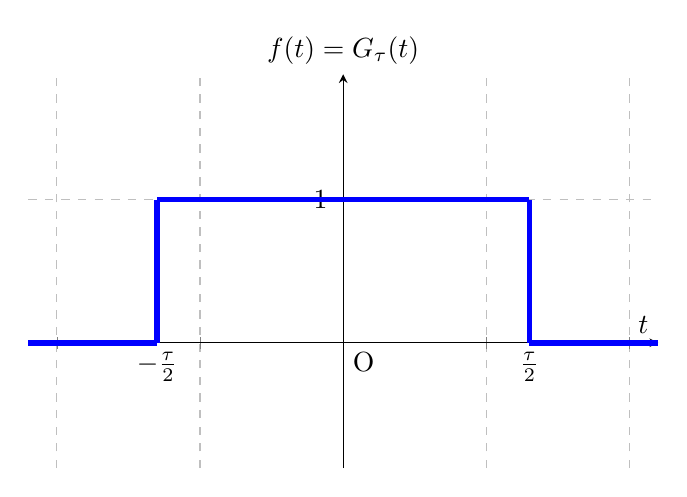
\begin{tikzpicture}
                \begin{axis}[
                    axis lines = middle,
                    xlabel = {$t$},
                    ylabel = {$f(t) = G_{\tau}(t)$},
                    ylabel style={at={(rel axis cs:0.5, 1)}, anchor=south},
                    xmin = -2.2, xmax = 2.2,
                    ymin = -0.2, ymax = 1.2,
                    xtick = {-2, -1, 0, 1, 2},
                    xticklabels = {$ $, $ $, $ $, $ $, $ $},
                    ytick distance = 1,
                    grid = major,
                    grid style = dashed,
                    scale only axis,
                    width = 8cm,
                    height = 5cm,
                    axis equal,
                ]
                \addplot[domain=-2.2:-1.3, samples=100, smooth, line width=2pt, blue] {0};
                \addplot[domain=-1.3:1.3, samples=100, smooth, line width=2pt, blue] {1};
                \addplot[domain=1.3:2.2, samples=100, smooth, line width=2pt, blue] {0};
                \addplot[smooth, line width=2pt, blue] coordinates {(-1.3, 0) (-1.3, 1)};
                \addplot[smooth, line width=2pt, blue] coordinates {(1.3, 1) (1.3, 0)};
                \node at (axis cs:0, 0) [anchor=north west] {O};
                \node at (axis cs:-1.3, 0) [anchor = north] {$-\frac{\tau}{2}$};
                \node at (axis cs:1.3, 0) [anchor = north] {$\frac{\tau}{2}$};
                \end{axis}
            \end{tikzpicture}
            \caption{$f(t)$ 的波形描述}
            \label{fig:rectangular-pulse-signal}
        \end{subfigure}
        \hfill
        \begin{subfigure}{0.45\textwidth}
            \centering
            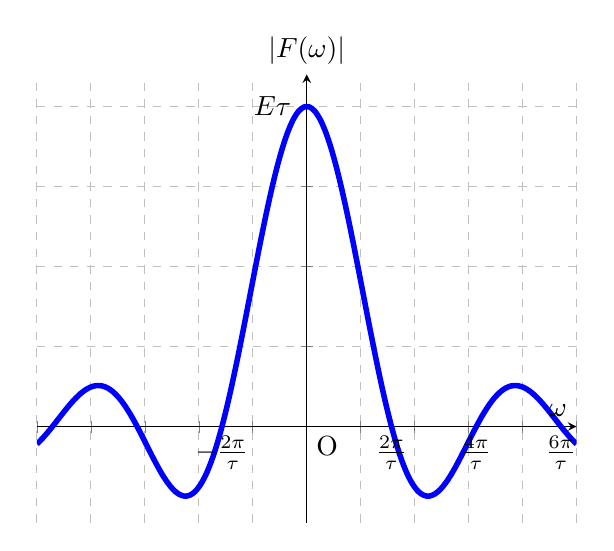
\begin{tikzpicture}
                \begin{axis}[
                    axis lines = middle,
                    xlabel = {$\omega$},
                    ylabel = {$|F(\omega)|$},
                    ylabel style={at={(rel axis cs:0.5, 1)}, anchor=south},
                    xmin = -10, xmax = 10,
                    ymin = -0.3, ymax = 1.1,
                    xtick = {-10, -8, -6, -4, -2, 0, 2, 4, 6, 8, 10},
                    xticklabels = {$ $, $ $, $ $, $ $, $ $, $ $, $ $, $ $, $ $, $ $, $ $},
                    ytick = {0, 0.25, 0.5, 0.75, 1},
                    yticklabels = {$ $, $ $, $ $, $ $, $E\tau$},
                    grid = major,
                    grid style = dashed,
                ]
                \addplot[domain=-10:10, samples=100, smooth, line width=2pt, blue] {sin(deg(x))/x};
                \node at (axis cs:0, 0) [anchor=north west] {O};
                \node at (axis cs:3.14, 0) [anchor = north] {$\frac{2\pi}{\tau}$};
                \node at (axis cs:-3.14, 0) [anchor = north] {$-\frac{2\pi}{\tau}$};
                \node at (axis cs:6.28, 0) [anchor = north] {$\frac{4\pi}{\tau}$};
                \node at (axis cs:9.42, 0) [anchor = north] {$\frac{6\pi}{\tau}$};
                \end{axis}
            \end{tikzpicture}
            \caption{$F(\omega)$ 的波形描述}
            \label{fig:rectangular-pulse-signal-ft}
        \end{subfigure}
        \caption{矩形脉冲信号及其傅里叶变换}
      \end{figure}
\end{theorem}

\begin{proof}
    由傅里叶变换的定义,有
    \begin{align*}
        F(\omega) & = \int_{-\infty}^{+\infty}EG_{\tau}(t)\mathe^{-\mathi\omega t}\D{t} \\
        & = E\int_{-\tau/2}^{\tau/2}\mathe^{-\mathi\omega t}\D{t} \\
        & = E\left.\frac{\mathe^{-\mathi\omega t}}{-\mathi\omega}\right|_{-\tau/2}^{\tau/2} \\
        & = \frac{E}{-\mathi\omega}\left(\mathe^{-\mathi\omega\tau/2} - \mathe^{\mathi\omega\tau/2}\right) \\
        & = \frac{E\cdot (-2\mathi\sin(\omega\tau/2))}{-\mathi\omega} \\
        & = E\tau\sa\left(\frac{\omega\tau}{2}\right).
    \end{align*}
    命题得证。
\end{proof}

\begin{property}[矩形脉冲信号的 FT 的特点]
    矩形脉冲信号的 FT 具有以下特点:
    \begin{itemize}
        \item FT 为 $\sa$ 函数,原点处函数值为矩形脉冲的面积 $E\tau$。
        \item FT 的零点为 $\omega = 2k\pi / \tau(k \in \set{Z}, k \neq 0)$。
        \item 频域的能量集中在第一个过零点区间,$[-2\pi/\tau, 2\pi/\tau]$。
        \item 带宽为 $B_\omega = 4\pi / \tau$,只与脉宽有关,与脉高无关。
    \end{itemize}
\end{property}

\subsubsection{冲激信号}

\begin{theorem}
    设有一个冲激信号 $f(t) = E\delta(t)$,则其傅里叶变换为
    \begin{align*}
        F(\omega) = \mathcal{F}[E\delta(t)] = E.
    \end{align*}
\end{theorem}

\begin{proof}
    由傅里叶变换的定义,有
    \begin{align*}
        F(\omega) & = \int_{-\infty}^{+\infty}E\delta(t)\mathe^{-\mathi\omega t}\D{t} \\
        & = E\mathe^{-\mathi\omega\cdot 0} \\
        & = E.
    \end{align*}
    命题得证。
\end{proof}

\begin{remark}
    上述结论也可以由矩形脉冲信号的极限情况得到。

    当脉宽 $\tau$ 逐渐变窄时,其频谱必然展宽。
    可以想象:$\delta(t)$ 积分为 $1$,因此需要 $E\tau = 1$。
    若 $\tau \to 0$,这时矩形脉冲就变成了 $\delta(t)$,
    其相应频谱 $F(\omega)$ 必定等于常数 $1$。
\end{remark}

\begin{definition}[均匀谱]
    冲激函数的频谱等于常数,即在整个频率范围内频谱是均匀分布的。
    
    显然,在时域中变化异常剧烈的冲激函数中包含了\bd{幅度相等}的\bd{所有}频率分布。
    因此,这种频谱常被称为\bd{均匀谱},或\bd{白色谱}。
\end{definition}

\begin{theorem}[常数的傅里叶变换]
    常数信号 $f(t) = E$ 的傅里叶变换为
    \begin{align*}
        F(\omega) = \mathcal{F}[E] = 2\pi\cdot E\delta(\omega).
    \end{align*}
    特别地,$\mathcal{F}[1/2\pi] = \delta(\omega), \mathcal{F}[1] = 2\pi\delta(\omega)$。
    这说明,直流信号的傅里叶频谱是位于零点的冲激函数。

    反之,冲激信号 $F(\omega) = E\delta(\omega)$ 的傅里叶逆变换为
    \begin{align*}
        f(t) = \mathcal{F}^{-1}[E\delta(\omega)] = \frac{E}{2\pi}.
    \end{align*}
    这说明,频谱零点处的冲激函数来自信号的直流分量。
\end{theorem}

\begin{proof}
    由于 $F[\mathe^{\mathi \omega_0 t}] = 2\pi\delta(\omega - \omega_0)$,
    故当 $\omega_0 = 0$ 时,有
    \begin{align*}
        F[1] = 2\pi\delta(\omega).
    \end{align*}
    又因为傅里叶变换是线性的,故有
    \begin{align*}
        F[E] = E\cdot F[1] = 2\pi\cdot E\delta(\omega).
    \end{align*}
    反之,由傅里叶逆变换的定义,有
    \begin{align*}
        f(t) = \mathcal{F}^{-1}[E\delta(\omega)] = \frac{E}{2\pi}.
    \end{align*}
    命题得证。
\end{proof}

\subsubsection{符号函数}

\begin{note}
    此节属于自己额外整理的内容,不在课程范围内。
\end{note}

\begin{theorem}
    设有一个符号函数 $f(t) = \sgn{t}$,则其傅里叶变换为
    \begin{align*}
        F(\omega) = \mathcal{F}[\sgn{t}] = \frac{2}{\mathi\omega}.
    \end{align*}
\end{theorem}

\begin{note}
    如果我们用傅里叶变换的定义来计算 $\sgn{t}$ 的傅里叶变换,我们会发现
    \begin{align*}
        F(\omega) & = \int_{-\infty}^{+\infty}\sgn{t}\mathe^{-\mathi\omega t}\D{t} \\
        & = - \int_{-\infty}^{0}\mathe^{-\mathi\omega t}\D{t} + \int_{0}^{+\infty}\mathe^{-\mathi\omega t}\D{t} \\
    \end{align*}
    这两个积分是不收敛的,因此我们需要用其他方法来计算 $\sgn{t}$ 的傅里叶变换。
\end{note}

\begin{proof}
    考虑使用指数函数信号来逼近符号函数,即
    \begin{align*}
        f_a(t) = \begin{cases}
            \mathe^{-at}, & t \ge 0, \\
            -\mathe^{at}, & t < 0,
        \end{cases}
        \quad a > 0.
    \end{align*}
    则符号函数可以表示为
    \begin{align*}
        \sgn{t} = \lim_{a \to 0^+}f_a(t).
    \end{align*}
    我们首先计算 $f_a(t)$ 的傅里叶变换:
    \begin{align*}
        F_a(\omega) & = \int_{-\infty}^{+\infty}f_a(t)\mathe^{-\mathi\omega t}\D{t} \\
        & = \int_{0}^{+\infty}\mathe^{-at}\mathe^{-\mathi\omega t}\D{t} + \int_{-\infty}^{0}-\mathe^{at}\mathe^{-\mathi\omega t}\D{t} \\
        & = \int_{0}^{+\infty}\mathe^{-(a + \mathi\omega)t}\D{t} - \int_{-\infty}^{0}\mathe^{(a - \mathi\omega)t}\D{t} \\
        & = \left.\frac{\mathe^{-(a + \mathi\omega)t}}{-(a + \mathi\omega)}\right|_{0}^{+\infty} - \left.\frac{\mathe^{(a - \mathi\omega)t}}{a - \mathi\omega}\right|_{-\infty}^{0} \\
        & = \frac{1}{a + \mathi\omega} - \frac{1}{a - \mathi\omega} \\
        & = -\frac{2\mathi\omega}{a^2 + \omega^2}.
    \end{align*}
    因此,有
    \begin{align*}
        F(\omega) = \lim_{a \to 0^+}F_a(\omega) = \lim_{a \to 0^+}\left(-\frac{2\mathi\omega}{a^2 + \omega^2}\right) = \frac{2}{\mathi\omega}.
    \end{align*}
    命题得证。
\end{proof}

\subsubsection{单位阶跃函数}

\begin{theorem}
    \label{thm:unit-step-function-ft}
    设有一个单位阶跃函数 $f(t) = u(t)$,则其傅里叶变换为
    \begin{align*}
        F(\omega) = \mathcal{F}[u(t)] = \frac{1}{\mathi\omega} + \pi\delta(\omega).
    \end{align*}
\end{theorem}

\begin{proof}
    由于
    \begin{align*}
        u(t) = \frac{1 + \sgn{t}}{2},
    \end{align*}
    故由傅里叶变换的线性性质,有
    \begin{align*}
        F(\omega) = \frac{1}{2}\mathcal{F}[1] + \frac{1}{2}\mathcal{F}[\sgn{t}] = \frac{1}{2}\cdot 2\pi\delta(\omega) + \frac{1}{2}\cdot \frac{2}{\mathi\omega} = \frac{1}{\mathi\omega} + \pi\delta(\omega).
    \end{align*}
    命题得证。
\end{proof}

\subsection{傅里叶变换的性质}

\subsubsection{FT 是线性运算}

\begin{property}
    设 $f(t)$ 和 $g(t)$ 是两个信号,$a$ 和 $b$ 是两个常数,
    且 $F(\omega)$ 和 $G(\omega)$ 分别是 $f(t)$ 和 $g(t)$ 的 FT,
    则有
    \begin{align*}
        \mathcal{F}[af(t) + bg(t)] = aF(\omega) + bG(\omega).
    \end{align*}
    这说明,对一个信号求 FT,等于对其分量(分信号)求 FT 然后再组合。
\end{property}

\begin{remark}
    FT 是线性运算,是因为 FT 既有\bd{齐次性},又有\bd{叠加性}。
    齐次性是指 $\mathcal{F}[af(t)] = a\mathcal{F}[f(t)]$,
    叠加性是指 $\mathcal{F}[f(t) + g(t)] = \mathcal{F}[f(t)] + \mathcal{F}[g(t)]$。
\end{remark}

\subsubsection{FT 的反褶和共轭的性质}

\begin{property}
    设信号 $f(t)$ 的 FT 为 $F(\omega)$,则进行反褶和共轭操作后的信号的 FT 对应关系如下:
    \begin{figure}[H]
        \begin{tabular}
            {c||c|c}
            操作 & 时域 & 频域 \\
            \hline
            反褶 & $f(-t)$ & $F(-\omega)$ \\
            共轭 & $f^*(t)$ & $F^*(-\omega)$ \\
            反褶且共轭 & $f^*(-t)$ & $F^*(\omega)$ \\
        \end{tabular}
    \end{figure}
\end{property}

\subsubsection{傅里叶变换及其逆变换的对偶性}

注意到 FT 和 IFT 在形式上极为相似:
\begin{align*}
    F(\omega) & = \quad\;\; \int_{-\infty}^{+\infty} f(t)\mathe^{-\mathi\omega t}\D{t}, \\
    f(t) & = \frac{1}{2\pi} \int_{-\infty}^{+\infty} F(\omega)\mathe^{\mathi\omega t}\D{\omega}.
\end{align*}
所以,我们可以尝试从这个切入点入手,来研究 FT 和 IFT 之间的关系。
FT 和 IFT 的变换核之间是共轭对称的。因此,IFT 可以由 FT 来完成。

\begin{lemma}[FT 和 IFT 的变换核之间的关系]
    FT 与 IFT 的变换核函数是共轭对称的,即
    \begin{align*}
        (\mathe^{-\mathi\omega t})^* = \mathe^{\mathi\omega t}, \quad
        (\mathe^{\mathi\omega t})^* = \mathe^{-\mathi\omega t}.
    \end{align*}
\end{lemma}

\begin{proof}
    由共轭的定义,我们有
    \begin{align*}
        (\mathe^{-\mathi\omega t})^* = (\cos\omega t - \mathi\sin\omega t)^* = \cos\omega t + \mathi\sin\omega t = \mathe^{\mathi\omega t}, \\
        (\mathe^{\mathi\omega t})^* = (\cos\omega t + \mathi\sin\omega t)^* = \cos\omega t - \mathi\sin\omega t = \mathe^{-\mathi\omega t}.
    \end{align*}
    命题得证。
\end{proof}

\begin{theorem}
    设 $f(t)$ 是一个信号,其 FT 为 $F(\omega)$,则有
    \begin{align*}
        \mathcal{F}^{-1}[F(\omega)] = f(t) = \frac{1}{2\pi}\{\mathcal{F}_{\omega}[F^*(\omega)]\}^*.
    \end{align*}
    其中 $\mathcal{F}_\omega(\cdot)$ 表示以 $\omega$ 为自变量求 FT,结果为 $t$ 的函数。
\end{theorem}

\begin{proof}
    根据 IFT 的定义,我们有
    \begin{align*}
        f(t) = \frac{1}{2\pi} \int_{-\infty}^{+\infty} F(\omega)\mathe^{\mathi\omega t}\D{\omega}.
    \end{align*}
    由于 FT 和 IFT 的变换核之间是共轭对称的,我们有
    \begin{align*}
        f(t) & = \frac{1}{2\pi} \int_{-\infty}^{+\infty} F(\omega)\mathe^{\mathi\omega t}\D{\omega} \\
        & = \frac{1}{2\pi} \int_{-\infty}^{+\infty} F(\omega)(\mathe^{-\mathi\omega t})^*\D{\omega} \\
        & = \frac{1}{2\pi} \left\{\int_{-\infty}^{+\infty} F^*(\omega)\mathe^{-\mathi\omega t}\D{\omega}\right\}^* \\
        & = \frac{1}{2\pi}\{\mathcal{F}_{\omega}[F^*(\omega)]\}^*.
    \end{align*}
    命题得证。
\end{proof}

\begin{property}
    设 $f(t)$ 是一个信号,其 FT 为 $F(\omega)$,则有
    \begin{align*}
        \mathcal{F}[F(t)] = 2\pi f(-\omega).
    \end{align*}
    注意,这里的 $F(t)$ 的自变量为 $t$,而 $f(-\omega)$ 的自变量为 $\omega$。
\end{property}

\begin{proof}
    由傅里叶逆变换的定义,有
    \begin{align*}
        f(t) = \frac{1}{2\pi}\int_{-\infty}^{+\infty} F(\omega)\mathe^{\mathi\omega t}\D{\omega},
    \end{align*}
    把 $\omega$ 和 $t$ 地位交换,有
    \begin{align*}
        f(\omega) = \frac{1}{2\pi}\int_{-\infty}^{+\infty} F(t)\mathe^{\mathi\omega t}\D{t}.
    \end{align*}
    令自变量为 $-\omega$,则
    \begin{align*}
        f(-\omega) = \frac{1}{2\pi}\int_{-\infty}^{+\infty} F(t)\mathe^{-\mathi\omega t}\D{t} = \frac{\mathcal{F}[F(t)]}{2\pi}.
    \end{align*}
    命题得证。
\end{proof}

\begin{property}
    设 $f(t)$ 是一个信号,其 FT 为 $F(\omega)$,则有
    \begin{align*}
        \mathcal{F}^{-1}[f(\omega)] = \frac{F(-t)}{2\pi}.
    \end{align*}
    注意,这里的 $f(\omega)$ 的自变量为 $\omega$,而 $F(-t)$ 的自变量为 $t$。
\end{property}

\begin{proof}
    由于 $\mathcal{F}[F(t)] = 2\pi f(-\omega)$,因此
    \begin{align*}
        \frac{1}{2\pi}F(t) = \mathcal{F}^{-1}[f(-\omega)],
    \end{align*}
    此即
    \begin{align*}
        \mathcal{F}^{-1}[f(\omega)] = \frac{F(-t)}{2\pi}.
    \end{align*}
    命题得证。
\end{proof}

\begin{corollary}
    当 $f(t)$ 为偶函数或奇函数时,FT 的对应关系为:
    \begin{itemize}
        \item 若 $f(t)$ 是偶函数,则 $F(t) \iff 2\pi f(\omega)$。
        \item 若 $f(t)$ 为奇函数,则 $F(t) \iff -2\pi f(\omega)$。
    \end{itemize}
\end{corollary}

\subsubsection{FT 的尺度变换特性}

\begin{property}
    设 $f(t)$ 是一个信号,其 FT 为 $F(\omega)$,则有
    \begin{align*}
        \mathcal{F}[f(at)] = \frac{1}{|a|}F\left(\frac{\omega}{a}\right), \quad a \neq 0.
    \end{align*}
    这说明,信号的压扩变换对函数的影响是相反的,同时幅度也会变化。
\end{property}

\begin{proof}
    根据 FT 的定义,有
    \begin{align*}
        \mathcal{F}[f(at)] = \int_{-\infty}^{+\infty} f(at)\mathe^{-\mathi\omega t}\D{t}.
    \end{align*}
    令 $u = at$,则有 $\D{u} = a\D{t}$,且 $t = u/a$,则有
    \begin{align*}
        \mathcal{F}[f(at)] = \frac{1}{|a|}\int_{-\infty}^{+\infty} f(u)\mathe^{-\mathi\omega u/a}\D{u} = \frac{1}{|a|}F\left(\frac{\omega}{a}\right).
    \end{align*}
    带绝对值是因为在 $a < 0$ 的情况下,积分上下限会发生变化。命题得证。
\end{proof}

\subsubsection{FT 图像的面积}

\begin{property}
    当 $f(t), F(\omega)$ 在 $(-\infty, +\infty)$ 上的积分存在时,有
    \begin{align*}
        F(0) & = \int_{-\infty}^{+\infty} f(t)\D{t}, \\
        f(0) & = \frac{1}{2\pi}\int_{-\infty}^{+\infty} F(\omega)\D{\omega}.
    \end{align*}
    这说明,$f(t)$ 与 $F(\omega)$ 所覆盖的面积,分别等于 $F(0)$ 和 $2\pi f(0)$。
\end{property}

\begin{proof}
    根据 FT 的定义,有
    \begin{align*}
        F(0) & = \int_{-\infty}^{+\infty} f(t)\mathe^{-\mathi\cdot 0 t}\D{t} = \int_{-\infty}^{+\infty} f(t)\D{t}, \\
        f(0) & = \frac{1}{2\pi}\int_{-\infty}^{+\infty} F(\omega)\mathe^{\mathi\cdot 0 \omega}\D{\omega} = \frac{1}{2\pi}\int_{-\infty}^{+\infty} F(\omega)\D{\omega}.
    \end{align*}
    命题得证。
\end{proof}

\begin{definition}[等效脉宽与等效带宽]
    不妨设 $f(0)$ 与 $F(0)$ 分别为各自函数的最大值,则定义信号的\bd{等效脉宽}与\bd{等效带宽}为
    \begin{align*}
        \tau & = \frac{F(0)}{f(0)}, \\
        B_\omega & = \frac{f(0)}{F(0)}.
    \end{align*}
\end{definition}

\begin{example}
    如图 \ref{fig:equivalent-bandwidth-and-pulse-width} 所示为
    偶双边指数信号 $f(t) = \mathe^{-a|t|}$ 及其频谱。
    图中标明了等效脉宽 $\tau$ 与等效带宽 $B_\omega$。
    \begin{figure}[H]
        \centering
        \includegraphics[width = 0.6\linewidth]{chap2/img/equivalent-bandwidth-and-pulse-width.png}
        \caption{等效脉宽与等效带宽}
        \label{fig:equivalent-bandwidth-and-pulse-width}
    \end{figure}
\end{example}

\begin{note}
    有时不特别区分频率和角频率,对 $B_f$ 与 $B_\omega$ 也不做特别区分。
\end{note}

\subsubsection{FT 的时移特性}

\begin{property}
    设信号 $f(t)$ 的 FT 为 $F(\omega)$,则有
    \begin{align*}
        \mathcal{F}[f(t - t_0)] = F(\omega)\mathe^{-\mathi\omega t_0}.
    \end{align*}
    时域延时,频域则是\bd{相位变化},不影响幅度谱,只在相位谱上叠加一个线性相位。

    与尺度变换结合,可以得到 $f(at - t_0)$ 的 FT 为
    \begin{align*}
        \mathcal{F}[f(at - t_0)] = \frac{1}{|a|}F\left(\frac{\omega}{a}\right)\mathe^{-\mathi\omega t_0/a}.
    \end{align*}
    因为 $f(at - t_0)$ 可以看做是 $f(t)$ 先向右平移 $t_0$ 个单位,再压扩 $a$ 倍得到的。
\end{property}

\begin{example}
    人耳通过相位信息差异,可以判定声音的远近变化。
    但声音信号的相位变化不影响内容上的理解。
\end{example}

\subsubsection{FT 的频移特性}

\begin{property}
    设信号 $f(t)$ 的 FT 为 $F(\omega)$,则有
    \begin{align*}
        \mathcal{F}[\mathe^{\mathi\omega_0 t}f(t)] = F(\omega - \omega_0).
    \end{align*}
    这说明,频域上的频移会导致时域上的相位变化。相位增加,频谱右移。

    与尺度变换结合,可以得到当 $a \neq 0$ 时,$\frac{1}{|a|}\mathe^{\mathi\omega_0 t/a}f(t/a)$ 的 FT 为
    \begin{align*}
        \mathcal{F}\left[\frac{1}{|a|}\mathe^{\mathi\omega_0 t/a}f(t/a)\right] = F(a\omega - \omega_0).
    \end{align*}
\end{property}

\begin{remark}
    理论上,时域信号乘以一个复指数信号,原信号的频谱将被搬移到复指数信号的频率处。
    实际应用中,利用欧拉公式,通过乘以\bd{正弦或余弦信号},也可以达到频谱搬移的目的。

    本质上,这都是因为 $\mathcal{F}[\mathe^{\mathi \omega_0 t}] = 2\pi\delta(\omega - \omega_0)$。
\end{remark}

\begin{note}
    有关 FT 的\bd{波形运算}的小结如下,设 $f(t) \iff F(\omega)$:
    \begin{itemize}
        \item 反褶:$f(-t) \iff F(-\omega)$。
        \item 平移:$f(t - t_0) \iff F(\omega)\mathe^{-\mathi\omega t_0}, F(\omega - \omega_0) \iff f(t)\mathe^{\mathi\omega_0 t}$。
    \end{itemize}
    即,时域延时,幅度谱不变;频谱搬移,通过在时域乘以复指数信号实现。
\end{note}

\subsubsection{FT 的微分与积分特性}

\begin{property}[微分特性]
    设 $f(t)$ 是一个信号,其 FT 为 $F(\omega)$,则有
    \begin{itemize}
        \item (时域微分)
            \begin{align*}
                \mathcal{F}\left[\frac{\D}{\D{t}}f(t)\right] = \mathi \omega F(\omega)
            \end{align*}
        \item (频域微分)
            \begin{align*}
                \mathcal{F}^{-1}\left[\frac{\D}{\D{\omega}}F(\omega)\right] = -\mathi t f(t)
            \end{align*}
    \end{itemize}
\end{property}

\begin{proof}
    由于
    \begin{align*}
        f(t) = \frac{1}{2\pi}\int_{-\infty}^{+\infty}F(\omega)\mathe^{\mathi \omega t}\D{\omega},
    \end{align*}
    对 $f(t)$ 求导,有
    \begin{align*}
        \dfrac{\D}{\D{t}}f(t) & = \dfrac{\D}{\D{t}}\left[\frac{1}{2\pi}\int_{-\infty}^{+\infty}F(\omega)\mathe^{\mathi \omega t}\D{\omega}\right] \\
        & = \mathi \omega \frac{1}{2\pi}\int_{-\infty}^{+\infty}F(\omega)\mathe^{\mathi \omega t}\D{\omega} \\
        & = \mathi \omega f(t).
    \end{align*}
    因此
    \begin{align*}
        \mathcal{F}\left[\frac{\D}{\D{t}}f(t)\right] = \mathcal{F}[\mathi \omega f(t)] = \mathi \omega F(\omega).
    \end{align*}
    同理,
    \begin{align*}
        F(\omega) = \int_{-\infty}^{+\infty}f(t)\mathe^{-\mathi \omega t}\D{t},
    \end{align*}
    对 $F(\omega)$ 求导,有
    \begin{align*}
        \dfrac{\D}{\D{\omega}}F(\omega) & = \dfrac{\D}{\D{\omega}}\left[\int_{-\infty}^{+\infty}f(t)\mathe^{-\mathi \omega t}\D{t}\right] \\
        & = -\mathi t \int_{-\infty}^{+\infty}f(t)\mathe^{-\mathi \omega t}\D{t} \\
        & = -\mathi t F(\omega).
    \end{align*}
    因此
    \begin{align*}
        \mathcal{F}^{-1}\left[\frac{\D}{\D{\omega}}F(\omega)\right] = \mathcal{F}^{-1}[-\mathi t F(\omega)] = -\mathi t f(t).
    \end{align*}
    命题得证。
\end{proof}

\begin{property}[积分特性]
    设 $f(t)$ 是一个信号,其 FT 为 $F(\omega)$,则有
    \begin{itemize}
        \item (时域积分)
            \begin{align*}
                \mathcal{F}\left[\int_{-\infty}^{t}f(\tau)\D{\tau}\right] = \frac{F(\omega)}{\mathi\omega} + \pi F(0)\delta(\omega)
            \end{align*}
        \item (频域积分)
            \begin{align*}
                \mathcal{F}^{-1}\left[\int_{-\infty}^{\omega}F(\lambda)\D{\lambda}\right] = \frac{f(t)}{-\mathi t} + \pi f(0)\delta(t)
            \end{align*}
    \end{itemize}
\end{property}

\begin{proof}
    记 $g(t) = \int_{-\infty}^{t}f(\tau)\D{\tau} - F(0)u(t)$,由于
    \begin{align*}
        F(0) = \int_{-\infty}^{+\infty}f(t)\D{t},
    \end{align*}
    则 $\lim_{t \to -\infty}g(t) = \lim_{t \to +\infty}g(t) = 0$。
    对 $g(t)$ 的定义式求微分,有
    \begin{align*}
        \frac{\D}{\D{t}}g(t) = f(t) - F(0)\delta(t).
    \end{align*}
    由于 FT 是线性运算,则
    \begin{align*}
        \mathcal{F}[g(t)] = \mathcal{F}\left[\int_{-\infty}^{t}f(\tau)\D{\tau}\right] - F(0)\mathcal{F}[u(t)].
    \end{align*}
    同时,
    \begin{align*}
        \mathcal{F}[\frac{\D}{\D{t}}g(t)] = F(\omega) - F(0)\mathcal{F}[\delta(t)].
    \end{align*}
    由微分性质得
    \begin{align*}
        \mathcal{F}[\frac{\D}{\D{t}}g(t)] = \mathi \omega \mathcal{F}[g(t)].
    \end{align*}
    在 \ref{thm:unit-step-function-ft} 中我们已经证明了
    \begin{align*}
        \mathcal{F}[u(t)] = \frac{1}{\mathi\omega} + \pi\delta(\omega).
    \end{align*}
    结合上述结论,我们有
    \begin{align*}
        \mathcal{F}\left[\int_{-\infty}^{t}f(\tau)\D{\tau}\right] & = \mathcal{F}[g(t)] + F(0)\mathcal{F}[u(t)] \\
        & = \frac{\mathcal{F}[\frac{\D}{\D{t}}g(t)]}{\mathi\omega} + F(0)\mathcal{F}[u(t)] \\
        & = \frac{F(\omega) - F(0)\mathcal{F}[\delta(t)]}{\mathi\omega} + F(0)\mathcal{F}[u(t)] \\
        & = \frac{F(\omega) - F(0)}{\mathi\omega} + F(0)\left(\frac{1}{\mathi\omega} + \pi\delta(\omega)\right) \\
        & = \frac{F(\omega)}{\mathi\omega} + \pi F(0)\delta(\omega).
    \end{align*}
    同理,记 $G(\omega) = \int_{-\infty}^{\omega}F(\lambda)\D{\lambda} - 2\pi f(0)u(\omega)$,由于
    \begin{align*}
        f(0) = \frac{1}{2\pi}\int_{-\infty}^{+\infty}F(\omega)\D{\omega},
    \end{align*}
    则 $\lim_{\omega \to -\infty}G(\omega) = \lim_{\omega \to +\infty}G(\omega) = 0$。
    对 $G(\omega)$ 的定义式求微分,有
    \begin{align*}
        \frac{\D}{\D{\omega}}G(\omega) = F(\omega) - 2\pi f(0)\delta(\omega).
    \end{align*}
    由于 IFT 也是线性运算,则
    \begin{align*}
        \mathcal{F}^{-1}[G(\omega)] = \mathcal{F}^{-1}\left[\int_{-\infty}^{\omega}F(\lambda)\D{\lambda}\right] - 2\pi f(0)\mathcal{F}^{-1}[u(\omega)].
    \end{align*}
    同时,
    \begin{align*}
        \mathcal{F}^{-1}[\frac{\D}{\D{\omega}}G(\omega)] = f(t) - f(0).
    \end{align*}
    由微分性质得
    \begin{align*}
        \mathcal{F}^{-1}[\frac{\D}{\D{\omega}}G(\omega)] = -\mathi t \mathcal{F}^{-1}[G(\omega)].
    \end{align*}
    由 FT 的对称性,我们有
    \begin{align*}
        \mathcal{F}^{-1}[u(\omega)] = -\frac{1}{2\pi \mathi t} + \frac{\delta(t)}{2}.
    \end{align*}
    结合上述结论,我们有
    \begin{align*}
        \mathcal{F}^{-1}\left[\int_{-\infty}^{\omega}F(\lambda)\D{\lambda}\right] & = \mathcal{F}^{-1}[G(\omega)] + 2\pi f(0)\mathcal{F}^{-1}[u(\omega)] \\
        & = \frac{\mathcal{F}^{-1}[\frac{\D}{\D{\omega}}G(\omega)]}{-\mathi t} + 2\pi f(0)\mathcal{F}^{-1}[u(\omega)] \\
        & = \frac{f(t) - f(0)}{-\mathi t} + 2\pi f(0)\left(-\frac{1}{2\pi \mathi t} + \frac{\delta(t)}{2}\right) \\
        & = \frac{f(t)}{-\mathi t} + \pi f(0)\delta(t).
    \end{align*}
    命题得证。
\end{proof}

\subsubsection{FT 的卷积特性}

\begin{theorem}[时域卷积定理]
    设有信号 $f_1(t)$ 和 $f_2(t)$,则有
    \begin{align*}
        \mathcal{F}[f_1(t) * f_2(t)] = \mathcal{F}[f_1(t)] \cdot \mathcal{F}[f_2(t)].
    \end{align*}
\end{theorem}

\begin{proof}
    根据卷积的定义,有
    \begin{align*}
        f_1(t) * f_2(t) = \int_{-\infty}^{+\infty} f_1(\tau)f_2(t - \tau)\D{\tau}.
    \end{align*}
    对上式两边同时求 FT,有
    \begin{align*}
        \mathcal{F}[f_1(t) * f_2(t)] & = \int_{-\infty}^{+\infty} \left[\int_{-\infty}^{+\infty} f_1(\tau)f_2(t - \tau)\D{\tau}\right]\mathe^{-\mathi\omega t}\D{t} \\
        & = \int_{-\infty}^{+\infty} f_1(\tau)\left[\int_{-\infty}^{+\infty} f_2(t - \tau)\mathe^{-\mathi\omega t}\D{t}\right]\D{\tau} \\
        & = \int_{-\infty}^{+\infty} f_1(\tau)\left[\int_{-\infty}^{+\infty} f_2(t)\mathe^{-\mathi\omega(t + \tau)}\D{t}\right]\D{\tau} \\
        & = \int_{-\infty}^{+\infty} f_1(\tau)\left[\int_{-\infty}^{+\infty} f_2(t)\mathe^{-\mathi\omega t}\D{t}\right]\mathe^{-\mathi\omega\tau}\D{\tau} \\
        & = \left[\int_{-\infty}^{+\infty} f_1(\tau)\mathe^{-\mathi\omega\tau}\D{\tau}\right]\left[\int_{-\infty}^{+\infty} f_2(t)\mathe^{-\mathi\omega t}\D{t}\right] \\
        & = \mathcal{F}[f_1(t)] \cdot \mathcal{F}[f_2(t)].
    \end{align*}
    命题得证。
\end{proof}

\begin{theorem}[频域卷积定理]
    设有信号 $f_1(t)$ 和 $f_2(t)$,则有
    \begin{align*}
        \mathcal{F}[f_1(t) \cdot f_2(t)] = \dfrac{1}{2\pi}\mathcal{F}[f_1(t)] * \mathcal{F}[f_2(t)].
    \end{align*}
\end{theorem}

\begin{proof}
    不妨设 $f_1(t)$ 和 $f_2(t)$ 的 FT 分别为 $F_1(\omega)$ 和 $F_2(\omega)$。
    根据卷积的定义,有
    \begin{align*}
        F_1(\omega) * F_2(\omega) = \int_{-\infty}^{+\infty} F_1(\eta)F_2(\omega - \eta)\D{\eta}.
    \end{align*}
    对上式两边同时求 IFT,有
    \begin{align*}
        \mathcal{F}^{-1}[F_1(\omega) * F_2(\omega)] & = \frac{1}{2\pi}\int_{-\infty}^{+\infty} \left[\int_{-\infty}^{+\infty} F_1(\eta)F_2(\omega - \eta)\D{\eta}\right]\mathe^{\mathi\omega t}\D{\omega} \\
        & = \frac{1}{2\pi}\int_{-\infty}^{+\infty} F_1(\eta)\left[\int_{-\infty}^{+\infty} F_2(\omega - \eta)\mathe^{\mathi\omega t}\D{\omega}\right]\D{\eta} \\
        & = \frac{1}{2\pi}\int_{-\infty}^{+\infty} F_1(\eta)\left[\int_{-\infty}^{+\infty} F_2(\omega)\mathe^{\mathi(\omega + \eta)t}\D{\omega}\right]\D{\eta} \\
        & = \frac{1}{2\pi}\int_{-\infty}^{+\infty} F_1(\eta)\left[\int_{-\infty}^{+\infty} F_2(\omega)\mathe^{\mathi\omega t}\D{\omega}\right]\mathe^{\mathi\eta t}\D{\eta} \\
        & = 2\pi\cdot\left[\frac{1}{2\pi}\int_{-\infty}^{+\infty} F_1(\eta)\mathe^{\mathi\eta t}\D{\eta}\right]\left[\frac{1}{2\pi}\int_{-\infty}^{+\infty} F_2(\omega)\mathe^{\mathi\omega t}\D{\omega}\right] \\
        & = 2\pi \mathcal{F}^{-1}[F_1(\omega)] \cdot \mathcal{F}^{-1}[F_2(\omega)] \\
        & = 2\pi f_1(t) \cdot f_2(t).
    \end{align*}
    对上式两边同时求 FT,有
    \begin{align*}
        F_1(\omega) * F_2(\omega) = \mathcal{F}[2\pi f_1(t) \cdot f_2(t)],
    \end{align*}
    即
    \begin{align*}
        \mathcal{F}[f_1(t) \cdot f_2(t)] = \frac{1}{2\pi}F_1(\omega) * F_2(\omega).
    \end{align*}
    命题得证。
\end{proof}

\begin{example}
    若信号在截取时,是使用``与矩形脉冲函数''相乘来实现的,
    即,设有信号 $f_1(t)$ 和 $f_2(t) = G_{\tau}(t)$,则
    \begin{align*}
        \mathcal{F}[f_1(t) \cdot f_2(t)] = \frac{1}{2\pi}\mathcal{F}[f_1(t)] * \mathcal{F}[f_2(t)] = \frac{1}{2\pi}\mathcal{F}[f_1(t)] * \tau\sa\left(\frac{\tau\omega}{2}\right).
    \end{align*}
\end{example}

\begin{remark}
    但实际情况下不存在理想的矩形信号。矩形信号边缘的跳变,将引起原信号的频谱产生畸变。
\end{remark}

\subsubsection{FT 时域上的相关性定理}

\begin{theorem}
    设信号 $f_1(t)$ 和 $f_2(t)$ 的 FT 分别为 $F_1(\omega)$ 和 $F_2(\omega)$,则有
    \begin{align*}
        \mathcal{F}[R_{f_1, f_2}(t)] = \mathcal{F}[f_1(t)] \cdot \mathcal{F}^*[f_2(t)].
    \end{align*}
    特别地,若 $f_2(t)$ 为实偶函数,则 $\mathcal{F}[R_{f_1, f_2}(t)] = F_1(\omega)F_2(\omega)$。

    自相关的 FT 定义为
    \begin{align*}
        \mathcal{F}[R_f(t)] = \mathcal{F}[f(t)] \cdot \mathcal{F}^*[f(t)] = \|\mathcal{F}[f(t)]\|^2.
    \end{align*}
    这说明信号自相关函数与其幅度谱平方,是一对傅里叶变换对。
\end{theorem}

\begin{proof}
    由相关运算和 FT 的时域卷积定理,以及 FT 的共轭性质,有
    \begin{align*}
        \mathcal{F}[R_{f_1, f_2}(t)] & = \mathcal{F}[f_1(t) * f_2^*(-t)] \\
        & = \mathcal{F}[f_1(t)] \cdot \mathcal{F}[f_2^*(-t)] \\
        & = \mathcal{F}[f_1(t)] \cdot \mathcal{F}^*[f_2(t)].
    \end{align*}
    命题得证。
\end{proof}

\subsubsection{FT 的帕斯瓦尔定理}

\begin{theorem}
    设 $f(t)$ 是一个时域上的信号,其傅里叶变换为 $F(\omega)$,则有
    \begin{align*}
        \int_{-\infty}^{+\infty} \|f(t)\|^2 \D{t}
        = \frac{1}{2\pi}\int_{-\infty}^{+\infty} \|F(\omega)\|^2 \D{\omega}
        = \int_{-\infty}^{+\infty}\|F(2\pi f)\|^2 \D{f}.
    \end{align*}
    这说明,信号的能量在时域和频域上是守恒的。
\end{theorem}

\subsection{采样与量化的概念}

\begin{definition}[采样]
    把模拟信号变成数字信号时,每隔一个时间间隔
    在模拟信号波形上抽取一个幅度值,这称之为\bd{采样}。
    这是在某些\bd{离散}的时间点上提取\bd{连续}时间信号值的过程。

    采样的时间间隔称为\bd{采样周期} $T_s$,
    其倒数称为\bd{采样频率} $f_s = 1/T_s$。
    $\omega_s = 2\pi / T_s$ 称为\bd{采样角频率}。
\end{definition}

\begin{remark}
    在不发生混淆的情况下,$\omega_s$ 可简称为采样频率。
\end{remark}

\subsubsection{时域采样和幅度量化}

时域采样和幅度量化是数字信号处理的两个基本步骤,
如图 \ref{fig:sampling}、\ref{fig:quantize-1} 和 \ref{fig:quantize-2} 所示。
\begin{figure}[H]
    \centering
    \begin{subfigure}{0.30\textwidth}
        \centering
        \includegraphics[width=\textwidth]{chap2/img/sampling.png}
        \caption{时域采样}
        \label{fig:sampling}
    \end{subfigure}
    \hfill
    \begin{subfigure}{0.30\textwidth}
        \centering
        \includegraphics[width=\textwidth]{chap2/img/quantize-1.png}
        \caption{幅度量化(数据收集)}
        \label{fig:quantize-1}
    \end{subfigure}
    \hfill
    \begin{subfigure}{0.30\textwidth}
        \centering
        \includegraphics[width=\textwidth]{chap2/img/quantize-2.png}
        \caption{幅度量化(数据离散化)}
        \label{fig:quantize-2}
    \end{subfigure}
    \caption{时域采样和幅度量化}
\end{figure}

\subsubsection{采样的频率与分辨率}

采样的频率与分辨率会影响到信号的还原质量。
\begin{itemize}
    \item 采样频率升高,信号的还原质量会提高;但需要更大的存储空间(带宽)和成本。
    \item 采样分辨率升高,也能提高信号的还原质量;但需要更大的存储空间(精度)和成本。
\end{itemize}
如图 \ref{fig:sampling-frequency} 和 \ref{fig:sampling-resolution} 所示。
\begin{figure}[H]
    \centering
    \begin{subfigure}{0.45\textwidth}
        \centering
        \includegraphics[width=\textwidth]{chap2/img/sampling-frequency.png}
        \caption{采样频率对信号还原的影响}
        \label{fig:sampling-frequency}
    \end{subfigure}
    \hfill
    \begin{subfigure}{0.45\textwidth}
        \centering
        \includegraphics[width=\textwidth]{chap2/img/sampling-resolution.png}
        \caption{采样分辨率对信号还原的影响}
        \label{fig:sampling-resolution}
    \end{subfigure}
    \caption{采样频率与分辨率}
\end{figure}

\subsubsection{采样的应用}

在日常生活中,常可以看到用离散时间信号表示连续时间信号的例子。
如照片、屏幕的画面等等。在一定条件下,可以用离散时间信号代替连续时间信号。

\begin{example}[CCD 芯片的光显微图]
    CCD 芯片用 VLSI 技术制造。被分为许多微小区,当光成像在 CCD 芯片上时,
    就在这些空间离散的像素点上被采样,而生成了离散空间图像信号,
    如图 \ref{fig:ccd-chip} 所示。
    \begin{figure}[H]
        \centering
        \includegraphics[width=0.45\textwidth]{chap2/img/ccd-chip.png}
        \caption{CCD 芯片的光显微图}
        \label{fig:ccd-chip}
    \end{figure}
\end{example}

\subsection{采样与采样定理}

研究连续时间信号与离散时间信号之间的关系时,我们最关心什么?
\begin{itemize}
    \item 在什么条件下,一个连续时间信号可以用它的离散时间样本
        来代替而不致丢失原有的信息?
    \item 如何从连续时间信号的离散时间样本不失真地
        恢复成原来的连续时间信号?
\end{itemize}

\subsubsection{采样的数学模型}

\begin{property}
    在没有任何条件限制的情况下,从连续时间信号采样
    所得到的样本序列\bd{不能}唯一地代表原来的连续时间信号。
\end{property}

\begin{example}
    如图 \ref{fig:counterexample-sampling} 所示,
    三个信号在 $t = -3T, -2T, -T, 0, T, 2T, 3T$ 处取样相等,
    但 $x_1(t) \neq x_2(t) \neq x_3(t)$。
    \begin{figure}[H]
        \centering
        \includegraphics[width=0.45\textwidth]{chap2/img/counterexample-sampling.png}
        \caption{采样不能唯一地代表原来的连续时间信号}
        \label{fig:counterexample-sampling}
    \end{figure}
\end{example}

\begin{definition}
    采样的数学模型如图 \ref{fig:sampling-math-model} 所示,
    其中 $p(t)$ 是采样脉冲,$P(\mathi \omega)$ 是 $p(t)$ 的傅里叶变换。
    \begin{figure}[H]
        \centering
        \begin{tikzpicture}
            \draw (0,0) circle (0.25);
        
            \draw[->] (-1.5,0) -- (-0.5,0);
            \draw[->] (0.5,0) -- (1.5,0);
            \draw[->] (0,-1.5) -- (0,-0.5);
        
            \node at (0,0) {$\times$};
            \node at (-2,0) {$x(t)$};
            \node at (2,0) {$x_p(t)$};
            \node at (0,-2) {$p(t)$};
        \end{tikzpicture}
        \caption{采样的数学模型}
        \label{fig:sampling-math-model}
    \end{figure}

    \begin{itemize}
        \item 在时域上,$x_p(t) = x(t)p(t)$。
        \item 在频域上,$X_p(\mathi \omega) = \frac{1}{2\pi}X(\mathi \omega) * P(\mathi \omega)$。
    \end{itemize}
    当采样为\bd{冲激串采样}(\bd{理想采样})时,
    \begin{align*}
        p(t) & = \sum_{n = -\infty}^{+\infty}\delta(t - nT_s), \\
        x_p(t) & = x(t)p(t) = \sum_{n = -\infty}^{+\infty}x(nT_s)\delta(t - nT_s),
    \end{align*}
    其中 $T_s$ 为采样间隔。
\end{definition}

\begin{example}
    如图 \ref{fig:impulse-sampling-time} 所示,
    为利用冲激串进行采样的信号 $x(t)$、$p(t)$ 与 $x_p(t)$,
    其中采样间隔 $T_s = T$。
    \begin{figure}[H]
        \centering
        \includegraphics[width=0.45\textwidth]{chap2/img/impulse-sampling-time.png}
        \caption{冲激串采样的信号 $x(t)$、$p(t)$ 与 $x_p(t)$}
        \label{fig:impulse-sampling-time}
    \end{figure}
\end{example}

\begin{property}
    冲激串信号 $p(t)$ 的傅里叶频谱 $\mathcal{F}[p(t)] = P(\mathi \omega)$ 为
    \begin{align*}
        P(\mathi \omega) = \frac{2\pi}{T_s}\sum_{n = -\infty}^{+\infty}\delta(\omega - \frac{2\pi}{T_s}n).
    \end{align*}
    \label{property:impulse-sampling-frequency-1}
\end{property}

\begin{proof}
    将周期信号 $p(t)$ 按照指数形式进行傅里叶展开,有
    \begin{align*}
        p(t) = \sum_{n = -\infty}^{+\infty}F_n\mathe^{\mathi n\omega_s t},
    \end{align*}
    其中 $\omega_s = 2\pi/T_s$。因此 $\mathcal{F}[p(t)]$ 可以写成
    \begin{align*}
        \mathcal{F}[p(t)] & = \int_{-\infty}^{+\infty}p(t)\mathe^{-\mathi\omega t}\D{t} \\
        & = \int_{-\infty}^{+\infty}\left(\sum_{n = -\infty}^{+\infty}F_n\mathe^{\mathi n\omega_s t}\right)\mathe^{-\mathi\omega t}\D{t} \\
        & = \sum_{n = -\infty}^{+\infty}F_n\int_{-\infty}^{+\infty}\mathe^{\mathi n\omega_s t}\mathe^{-\mathi\omega t}\D{t},
    \end{align*}
    其中 $\int_{-\infty}^{+\infty}\mathe^{\mathi n\omega_s t}\mathe^{-\mathi\omega t}\D{t}
        = \mathcal{F}[\mathe^{\mathi n\omega_s t}] = 2\pi\delta(\omega - n\omega_s)$。
    所以
    \begin{align*}
        \mathcal{F}[p(t)] = \sum_{n = -\infty}^{+\infty}F_n2\pi\delta(\omega - n\omega_s).
    \end{align*}
    由傅里叶展开的定义知
    \begin{align*}
        F_n & = \frac{1}{T_s}\int_{-T_s/2}^{T_s/2}p(t)\mathe^{-\mathi n\omega_s t}\D{t} \\
        & = \frac{1}{T_s}\int_{-T_s/2}^{T_s/2}\sum_{n = -\infty}^{+\infty}\delta(t - nT_s)\mathe^{-\mathi n\omega_s t}\D{t}.
    \end{align*}
    在积分区间 $[-T_s/2, T_s/2]$ 内,只有 $t = 0$ 满足 $t$ 可以被写成 $t = nT_s$ 的形式,所以
    \begin{align*}
        F_n & = \frac{1}{T_s}\int_{-T_s/2}^{T_s/2}p(t)\mathe^{-\mathi n\omega_s t}\D{t} \\
        & = \frac{1}{T_s}\left.\left(p(t)\mathe^{-\mathi n\omega_s t}\right)\right|_{t = 0} \\
        & = \frac{1}{T_s}.
    \end{align*}
    故
    \begin{align*}
        P(\mathi \omega) & = \frac{1}{T_s}\sum_{n = -\infty}^{+\infty}2\pi\delta(\omega - n\omega_s) \\
        & = \frac{2\pi}{T_s}\sum_{n = -\infty}^{+\infty}\delta(\omega - \frac{2\pi}{T_s}n).
    \end{align*}
    命题得证。
\end{proof}

\begin{property}
    冲激串采样后的信号 $x_p(t)$ 的频谱 $\mathcal{F}[x_p(t)] = X_p(\mathi \omega)$ 为
    \begin{align*}
        X_p(\mathi \omega) = \frac{1}{T_s}\sum_{k = -\infty}^{+\infty}X(\mathi(\omega - k\omega_s)).
    \end{align*}
    \label{property:impulse-sampling-frequency-2}
\end{property}

\begin{proof}
    由采样的数学模型知
    \begin{align*}
        X_p(\mathi \omega) & = \frac{1}{2\pi}X(\mathi \omega) * P(\mathi \omega) \\
        & = \frac{1}{2\pi}X(\mathi \omega) * \left(\frac{2\pi}{T_s}\sum_{k = -\infty}^{+\infty}\delta(\omega - \frac{2\pi}{T_s}k)\right) \\
        & = \frac{1}{T_s}\sum_{k = -\infty}^{+\infty}X(\mathi \omega) * \delta(\omega - \frac{2\pi}{T_s}k) \\
        & = \frac{1}{T_s}\sum_{k = -\infty}^{+\infty}X(\mathi(\omega - k\omega_s)),
    \end{align*}
    其中 $\omega_s = 2\pi/T_s$,为采样频率。
\end{proof}

\begin{remark}
    由此可见,在时域对连续时间信号进行理想采样,
    就相当于在频域将连续时间信号的频谱\bd{以 $\omega_s$ 为周期进行延拓}。
\end{remark}

\begin{example}
    如图 \ref{fig:impulse-sampling-frequency} 所示,
    为利用冲激串进行采样的信号 $X(\mathi \omega)$、$P(\mathi \omega)$ 与 $X_p(\mathi \omega)$,
    其中采样频率 $\omega_s = 2\pi/T$。
    \begin{figure}[H]
        \centering
        \includegraphics[width=0.45\textwidth]{chap2/img/impulse-sampling-frequency.png}
        \caption{冲激串采样的信号 $X(\mathi \omega)$、$P(\mathi \omega)$ 与 $X_p(\mathi \omega)$}
        \label{fig:impulse-sampling-frequency}
    \end{figure}
\end{example}

\begin{exercise}
    现有信号 $f(t) = \mathe^{-t^2/20}$。为分析某时刻下的``局部频谱'',
    可选合适的窗函数 $w(t, t_0)$,并截取 $f(t)$ 在 $t_0$ 附近的信号,
    即 $f_w(t, t_0) = f(t)\cdot w(t, t_0)$。
    \begin{enumerate}[label=(\arabic*)]
        \item 求信号 $f(t)$ 的 FT。
        \item 现不妨取窗函数 $w(t, t_0) = \mathe^{-(t - t_0)^2/2}$。
            试分析 $t_0 = 0$ 时刻下对应的``局部频谱'',即求 $f_w(t, 0)$ 的 FT。
        \item 画出信号 $f(t)$ 的频谱图与信号 $f(t)$ 在 $t_0 = 0$ 时刻下的
            ``局部频谱''图,并进行对比。
    \end{enumerate}
    (提示:若 $x, c \in \set{R}$,则 $\int_{-\infty}^{+\infty}\mathe^{-(x + \mathi c)^2}\D{x} = \sqrt{\pi}$。)
\end{exercise}

\begin{solution}
    \begin{enumerate}[label=(\arabic*)]
        \item 不妨记 $f(t)$ 的 FT 为 $F(\omega)$。由傅里叶变换的定义知
            \begin{align*}
                F(\omega) & = \mathcal{F}[f(t)] = \int_{-\infty}^{+\infty} f(t)\mathe^{-\mathi\omega t}\D{t} \\
                & = \int_{-\infty}^{+\infty} \mathe^{-t^2/20}\mathe^{-\mathi\omega t}\D{t} \\
                & = \mathe^{-5\omega^2}\int_{-\infty}^{+\infty} \mathe^{-\frac{(t + 10\mathi \omega)^2}{20}}\D{t} \\
                & = 2\sqrt{5\pi}\mathe^{-5\omega^2}.
            \end{align*}
        \item 不妨记 $f_w(t, 0)$ 的 FT 为 $F_w(\omega, 0)$。由题知
            \begin{align*}
                f_w(t, 0) = f(t)\cdot w(t, 0) = \mathe^{-t^2/20}\mathe^{-t^2/2} = \mathe^{-\frac{11}{20}t^2}.
            \end{align*}
            因此,其傅里叶变换为
            \begin{align*}
                F_w(\omega, 0) & = \mathcal{F}[f_w(t, 0)] = \int_{-\infty}^{+\infty} f_w(t, 0)\mathe^{-\mathi\omega t}\D{t} \\
                & = \int_{-\infty}^{+\infty} \mathe^{-\frac{11}{20}t^2}\mathe^{-\mathi\omega t}\D{t} \\
                & = \mathe^{-\frac{5}{11}\omega^2}\int_{-\infty}^{+\infty} \mathe^{-\frac{11}{20}\left(t + \frac{10}{11}\mathi \omega\right)^2}\D{t} \\
                & = \frac{2}{11}\sqrt{55\pi}\mathe^{-\frac{5}{11}\omega^2}.
            \end{align*}
        \item 画出两者的频谱图如 \ref{fig:chap2-part6-exercise1-solution} 所示。
            \begin{figure}[H]
                \centering
                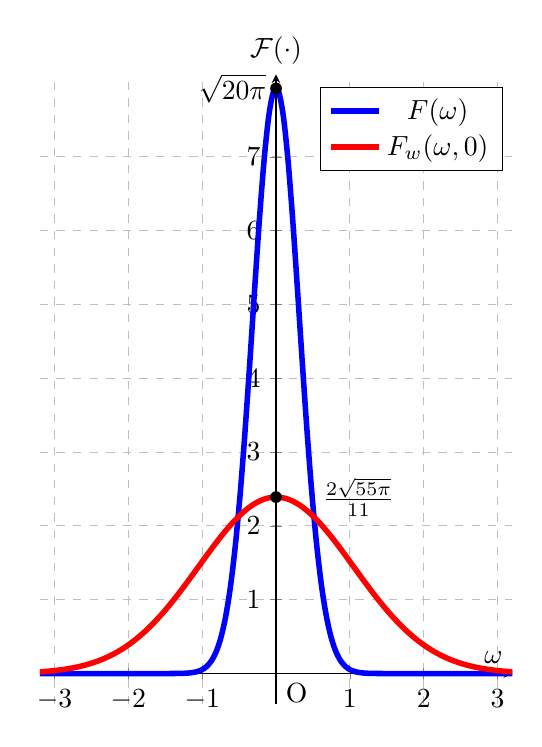
\begin{tikzpicture}
                    \begin{axis}[
                        axis lines = middle,
                        xlabel = {$\omega$},
                        ylabel = {$\mathcal{F}(\cdot)$},
                        ylabel style={at={(rel axis cs:0.5, 1)}, anchor=south},
                        xmin = -3.2, xmax = 3.2,
                        ymin = -0.2, ymax = 7.9,
                        xtick distance = 1,
                        ytick = {1, 2, 3, 4, 5, 6, 7},
                        grid = major,
                        grid style = dashed,
                        scale only axis,
                        width = 6cm,
                        height = 8cm,
                        axis equal,
                    ]
                    \addplot[domain=-3.2:3.2, samples=100, smooth, line width=2pt, blue] {sqrt(20 * pi) * exp(-5 * x^2)};
                    \addlegendentry{$F(\omega)$}
                    \addplot[domain=-3.2:3.2, samples=100, smooth, line width=2pt, red] {sqrt(20 / 11 * pi) * exp(-5 / 11 * x^2)};
                    \addlegendentry{$F_w(\omega, 0)$}
                    \node at (axis cs:0, 0) [anchor=north west] {O};
                    \node[circle, fill, inner sep=1.5pt] at (axis cs:0, 7.927) {};
                    \node at (axis cs:0, 7.927) [anchor=east] {$\sqrt{20\pi}$};
                    \node[circle, fill, inner sep=1.5pt] at (axis cs:0, 2.390) {};
                    \node at (axis cs:0.5, 2.390) [anchor=west] {$\frac{2\sqrt{55\pi}}{11}$};
                    \end{axis}
                \end{tikzpicture}
                \caption{频谱图像对比}
                \label{fig:chap2-part6-exercise1-solution}
            \end{figure}
            可以看出,这两个频率谱在 $\omega = 0$ 处均有峰值,但 $F(\omega)$ 的峰值更高,
            为 $F_w(\omega, 0)$ 的 $\sqrt{11}$ 倍。同时,$F_w(\omega, 0)$ 比 $F(\omega)$ 更加
            ``平缓'',即 $F_w(\omega, 0)$ 的峰值附近的值相对于峰值更小。
    \end{enumerate}
\end{solution}

\subsubsection{采样与混叠}

\begin{definition}[混叠]
    当采样周期变大时,频谱的周期会变小。此时,离散信号的谱会发生相互重叠的现象。
    这种现象称为\bd{混叠}。
\end{definition}

\begin{example}
    如图 \ref{fig:aliasing-example-1} 和 \ref{fig:aliasing-example-2} 所示,
    当采样频率 $T_s$ 变大时,信号 $F_s(\omega)$ 会发生混叠。
    \begin{figure}[H]
        \centering
        \begin{subfigure}{0.45\textwidth}
            \centering
            \includegraphics[width=\textwidth]{chap2/img/aliasing-example-1.png}
            \caption{采样频率 $T_s$ 较小}
            \label{fig:aliasing-example-1}
        \end{subfigure}
        \hfill
        \begin{subfigure}{0.45\textwidth}
            \centering
            \includegraphics[width=\textwidth]{chap2/img/aliasing-example-2.png}
            \caption{采样频率 $T_s$ 较大}
            \label{fig:aliasing-example-2}
        \end{subfigure}
        \caption{混叠现象}
    \end{figure}
\end{example}

\begin{example}
    设如图 \ref{fig:aliasing-example-3} 所示的模拟音频信号
    高频截止频率为 $f_M = 5\;\mathrm{kHz}$,采样频率为 $6\;\mathrm{kHz}$。
    问:采样后信号频谱与原信号频谱在 $2\;\mathrm{kHz}$ 处有什么差异?
    \begin{figure}[H]
        \centering
        \includegraphics[width=0.8\textwidth]{chap2/img/aliasing-example-3.png}
        \caption{模拟音频信号的频谱}
        \label{fig:aliasing-example-3}
    \end{figure}
\end{example}

\begin{solution}
    采样后的频谱相当于原信号的频谱以 $6\;\mathrm{kHz}$ 为周期进行叠加。
    在 $2\;\mathrm{kHz}$ 处的频谱为原 $2\;\mathrm{kHz}$ 处的频谱
    与 $4\;\mathrm{kHz}$ 处的频谱的混叠。
    幅度大小变为原来的 $1/T_s = 6000$ 倍。
    画出采样后的频谱如图 \ref{fig:aliasing-example-4} 所示。
    \begin{figure}[H]
        \centering
        \includegraphics[width=0.8\textwidth]{chap2/img/aliasing-example-4.png}
        \caption{采样后信号的频谱}
        \label{fig:aliasing-example-4}
    \end{figure}
\end{solution}

\begin{note}
    虽然图 \ref{fig:aliasing-example-4} 和图 \ref{fig:aliasing-example-3} 的
    频谱图像极为相似,但纵轴的幅度并不一样,前者是后者的 $1/T_s = 6000$ 倍。
\end{note}

\begin{example}
    设一模拟音频信号高频截止频率为 $10\;\mathrm{kHz}$。
    若采样频率为 $16\;\mathrm{kHz}$,
    则采样后信号频谱与原信号频谱在 $12\;\mathrm{kHz}$ 处有什么差异?
\end{example}

\begin{note}
    \bd{实信号}通过傅里叶变换后得到的频谱是关于 $f = 0$ 轴对称的,
    也就是\bd{双边频谱}。这是题目提到\bd{模拟信号/实信号}时需要
    下意识反应到的一个点。
\end{note}

\begin{solution}
    采样后的频谱相当于原信号的频谱以 $16\;\mathrm{kHz}$ 为周期进行叠加。
    在 $12\;\mathrm{kHz}$ 处的频谱为原 $-4\;\mathrm{kHz}$ 处
    (对称后,$4\;\mathrm{kHz}$ 处)的频谱。
    幅度大小变为原来的 $1/T_s = 16000$ 倍。
    因此
    \begin{align*}
        X_s(12\;\mathrm{kHz}) & = \frac{1}{T_s}X(-4\;\mathrm{kHz}) \\
        & = 16000X(4\;\mathrm{kHz}).
    \end{align*}
    信号会发生混叠,但混叠对 $12\;\mathrm{kHz}$ 处的频率分量没有影响。
\end{solution}

\begin{example}
    模拟信号(实信号)频率在 $850\;\mathrm{kHz}$ 到 $900\;\mathrm{kHz}$。
    若采样频率为 $200\;\mathrm{kHz}$,则采样后信号频谱在 $20\;\mathrm{kHz}$ 处
    与原信号有什么差异?
    (要求:文字说明幅度的变化;如果有混叠发生,请说明混叠对应的原频谱)
\end{example}

\begin{solution}
    由于采样频率 $\omega_s = 200\;\mathrm{kHz} > 2\Delta\omega = 100\;\mathrm{kHz}$,
    故不会发生混叠。采样后信号频谱在 $20\;\mathrm{kHz}$ 处的幅度为原信号频谱在
    $1020\;\mathrm{kHz}$ 处的幅度,为 $0$。
\end{solution}

\begin{remark}
    对于一个经过调制后的信号,若想要将其完整的恢复出来,也可以对其进行采样,
    然后过低通滤波器(其实就是解调的过程)。在这个过程中,
    当采样频率满足特定频率的时候,不需要其很高的采样频率也能将信号复原。
\end{remark}

\subsubsection{采样定理}

那么如何防止混叠现象的发生呢?我们以此为出发点,引出\bd{采样定理}。

要想使采样后的信号样本能完全代表原来的信号,
就意味着要能够从 $X_p(\mathi \omega)$中不失真地分离出 $X(\mathi \omega)$。
这就要求 $X(\mathi \omega)$ 在周期性延拓时不能发生频谱的混叠。
为此必须要求:
\begin{enumerate}
    \item $x(t)$ 必须是带限的,最高频率为 $\omega_M$。
    \item 采样间隔(周期)不是任意的,必须保证采样频率 $\omega_s \ge 2\omega_M$。
\end{enumerate}
在满足上述要求时,可以通过理想低通滤波器从 $X_p(\mathi \omega)$ 中
不失真地分离出 $X(\mathi \omega)$。

\begin{theorem}[Nyquist 采样定理]
    设 $x(t)$ 是带限信号,其最高频率为 $\omega_M$。
    如果以 $\omega_s > 2\omega_M$ 的频率进行采样,则 $x(t)$ 可以唯一地
    由其样本 $x(nT_s)$ 决定,其中 $T_s = 2\pi/\omega_s$。
\end{theorem}

\begin{example}[采样定理的图示]
    如图 \ref{fig:sampling-theorem} 所示为两种不同的采样频率 $\omega_s$ 下的采样效果。
    其中 $\omega_c$ 为过渡带的截止频率。
    \begin{itemize}
        \item 当 $\omega_s > 2\omega_M$ 时,采样后的频谱不会发生混叠,过渡带将两个周期的频谱分开。
        \item 当 $\omega_s < 2\omega_M$ 时,采样后的频谱会发生混叠,过渡带处两个周期的频谱混合在一起。
    \end{itemize}
    \begin{figure}[H]
        \centering
        \includegraphics[width=0.45\textwidth]{chap2/img/sampling-theorem.png}
        \caption{采样定理的图示}
        \label{fig:sampling-theorem}
    \end{figure}
\end{example}

\begin{example}
    在工程实际应用中,理想滤波器是不可能实现的。而非理想滤波器一定有过渡带,
    也就是如图 \ref{fig:real-sampling-theorem} 所示中
    的 $\omega_c \in (\omega_M, \omega_s - \omega_M)$。
    因此,实际采样时,$\omega_s$ 必须大于 $2\omega_M$。
    \begin{figure}[H]
        \centering
        \begin{subfigure}{0.45\textwidth}
            \centering
            \includegraphics[width=\textwidth]{chap2/img/real-sampling-theorem.png}
            \caption{实际情况下的采样定理的图示}
            \label{fig:real-sampling-theorem}
        \end{subfigure}
        \hfill
        \begin{subfigure}{0.45\textwidth}
            \centering
            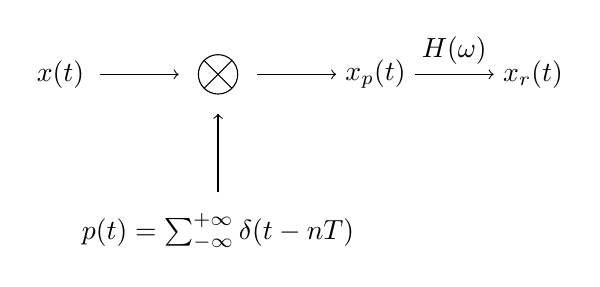
\begin{tikzpicture}
                \draw (0,0) circle (0.25);
            
                \draw (-0.177,-0.177) -- (0.177,0.177);
                \draw (0.177,-0.177) -- (-0.177,0.177);
            
                \draw[->] (-1.5,0) -- (-0.5,0);
                \draw[->] (0.5,0) -- (1.5,0);
                \draw[->] (0,-1.5) -- (0,-0.5);
                \draw[->] (2.5,0) -- (3.5,0) node[midway,above] {$H(\mathi\omega)$};
            
                \node at (-2,0) {$x(t)$};
                \node at (2,0) {$x_p(t)$};
                \node at (0,-2) {$p(t) = \sum_{-\infty}^{+\infty}\delta(t - nT)$};
                \node at (4,0) {$x_r(t)$};
            \end{tikzpicture}
            \caption{实际情况下的采样定理的数学模型}
            \label{fig:real-sampling-theorem-math-model}
        \end{subfigure}
        \caption{实际情况下的采样定理}
    \end{figure}
\end{example}

\subsubsection{采样定理的方法论思考}

采样定理的核心是如何通过对原始信号较少的\bd{采样}(选择局部),
来还原\bd{原信号}(体现整体)的全部知识,这也是人们通过数字信号,
进一步计算机,来表示真实世界模拟信号的方式。\bd{采样定理}就给出了
这种情况下对\bd{采样频率}的约束。

\begin{figure}[H]
    \begin{tikzpicture}
        \node at (4,2) [text width=7cm] (title) {多媒体计算机智能处理与应用};
        \node at (-2,0)[text width=5cm] (analog) {模拟(连续)世界};
        \node at (4,0)[text width=5cm] (digital) {数字(离散)世界};

        \draw[->] (-1.5,0) -- (1.5,0)
        node[midway, above] {采样} 
        node[midway, below] {桥梁};
        
        \draw[->] (3,0.5) -- (3,1.5)
        node[midway, right] {提取特征、改变特征};
    \end{tikzpicture}
\end{figure}

\subsubsection{内插}

\begin{definition}[理想低通滤波器]
    \bd{理想低通滤波器}是指频域上矩形脉冲 $H(\mathi\omega)$,
    如图 \ref{fig:ideal-low-pass-filter-magnitude} 和 \ref{fig:ideal-low-pass-filter-argument} 所示。
    \begin{align*}
        H(\mathi\omega) = \begin{cases}
            \mathe^{-\mathi\omega t_0}, & |\omega| \le \omega_c, \\
            0, & |\omega| > \omega_c.
        \end{cases}
    \end{align*}
    其单位冲激响应如图 \ref{fig:ideal-low-pass-filter-impulse-response} 所示,为
    \begin{align*}
        h(t) = \frac{\omega_c}{\pi}\sa{\left(\omega_c(t - t_0)\right)}.
    \end{align*}
    理想低通滤波器的单位冲激响应 $h(t)$,即为其傅里叶逆变换。
    \begin{figure}[H]
        \centering
        \begin{subfigure}{0.3\textwidth}
            \centering
            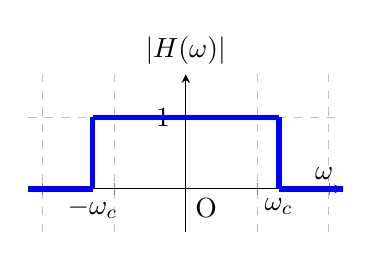
\begin{tikzpicture}
                \begin{axis}[
                    axis lines = middle,
                    xlabel = {$\omega$},
                    ylabel = {$|H(\mathi\omega)|$},
                    ylabel style={at={(rel axis cs:0.5, 1)}, anchor=south},
                    xmin = -2.2, xmax = 2.2,
                    ymin = -0.2, ymax = 1.2,
                    xtick = {-2, -1, 0, 1, 2},
                    xticklabels = {$ $, $ $, $ $, $ $, $ $},
                    ytick distance = 1,
                    grid = major,
                    grid style = dashed,
                    scale only axis,
                    width = 4cm,
                    height = 2cm,
                    axis equal,
                ]
                \addplot[domain=-2.2:-1.3, samples=100, smooth, line width=2pt, blue] {0};
                \addplot[domain=-1.3:1.3, samples=100, smooth, line width=2pt, blue] {1};
                \addplot[domain=1.3:2.2, samples=100, smooth, line width=2pt, blue] {0};
                \addplot[smooth, line width=2pt, blue] coordinates {(-1.3, 0) (-1.3, 1)};
                \addplot[smooth, line width=2pt, blue] coordinates {(1.3, 1) (1.3, 0)};
                \node at (axis cs:0, 0) [anchor=north west] {O};
                \node at (axis cs:-1.3, 0) [anchor = north] {$-\omega_c$};
                \node at (axis cs:1.3, 0) [anchor = north] {$\omega_c$};
                \end{axis}
            \end{tikzpicture}
            \caption{$|H(\mathi\omega)|$}
            \label{fig:ideal-low-pass-filter-magnitude}
        \end{subfigure}
        \hfill
        \begin{subfigure}{0.3\textwidth}
            \centering
            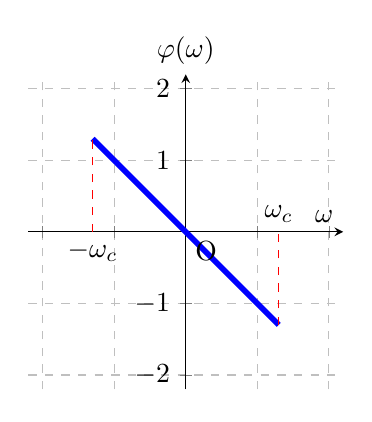
\begin{tikzpicture}
                \begin{axis}[
                    axis lines = middle,
                    xlabel = {$\omega$},
                    ylabel = {$\varphi(\omega)$},
                    ylabel style={at={(rel axis cs:0.5, 1)}, anchor=south},
                    xmin = -2.2, xmax = 2.2,
                    ymin = -1.2, ymax = 1.2,
                    xtick = {-2, -1, 0, 1, 2},
                    xticklabels = {$ $, $ $, $ $, $ $, $ $},
                    ytick distance = 1,
                    grid = major,
                    grid style = dashed,
                    scale only axis,
                    width = 4cm,
                    height = 4cm,
                    axis equal,
                ]
                \addplot[domain=-1.3:1.3, samples=100, smooth, line width=2pt, blue] {-x};
                \addplot[dashed, red] coordinates {(-1.3, 0) (-1.3, 1.3)};
                \addplot[dashed, red] coordinates {(1.3, -1.3) (1.3, 0)};
                \node at (axis cs:0, 0) [anchor=north west] {O};
                \node at (axis cs:-1.3, 0) [anchor = north] {$-\omega_c$};
                \node at (axis cs:1.3, 0) [anchor = south] {$\omega_c$};
                \end{axis}
            \end{tikzpicture}
            \caption{$\varphi(\omega)$}
            \label{fig:ideal-low-pass-filter-argument}
        \end{subfigure}
        \hfill
        \begin{subfigure}{0.3\textwidth}
            \centering
            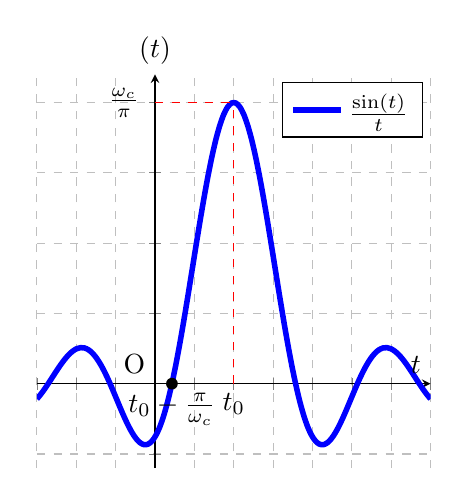
\begin{tikzpicture}
                \begin{axis}[
                    axis lines = middle,
                    xlabel = {$t$},
                    ylabel = {$\sa(t)$},
                    ylabel style={at={(rel axis cs:0.3, 1)}, anchor=south},
                    xmin = -6, xmax = 14,
                    ymin = -0.3, ymax = 1.1,
                    xtick = {-6, -4, -2, 0, 2, 4, 6, 8, 10, 12, 14},
                    xticklabels = {$ $, $ $, $ $, $ $, $ $, $ $, $ $, $ $, $ $, $ $, $ $},
                    ytick = {-0.25, 0, 0.25, 0.5, 0.75, 1},
                    yticklabels = {$ $, $ $, $ $, $ $, $ $, $\frac{\omega_c}{\pi}$},
                    grid = major,
                    grid style = dashed,
                    scale only axis,
                    width = 5cm,
                    height = 5cm,
                ]
                \addplot[domain=-6:14, samples=100, smooth, line width=2pt, blue] {sin(deg(x-4))/(x-4)};
                \addlegendentry{$\frac{\sin(t)}{t}$}
                \addplot[dashed, red] coordinates {(0, 1) (4, 1)};
                \addplot[dashed, red] coordinates {(4, 0) (4, 1)};
                \node at (axis cs:0, 0) [anchor=south east] {O};
                \node[circle, fill, inner sep=1.5pt] at (axis cs:0.86, 0) {};
                \node at (axis cs:0.86, 0) [anchor=north] {$t_0 - \frac{\pi}{\omega_c}$};
                \node at (axis cs:4, 0) [anchor=north] {$t_0$};
                \end{axis}
            \end{tikzpicture}
            \caption{$h(t) = \frac{\omega_c}{\pi}\cdot\sa{\left(\omega_c(t - t_0)\right)}$}
            \label{fig:ideal-low-pass-filter-impulse-response}
        \end{subfigure}
        \caption{理想低通滤波器}
    \end{figure}
\end{definition}

\begin{definition}[内插]
    \bd{内插}是指由样本值重建某一函数的过程。若原始信号是带限的,
    即信号的频谱宽度有限,则称之为\bd{带限内插}。

    如何恢复原始的时间连续信号?
    用滤波器函数对信号采样值进行内插来重建模拟信号,相当于滤波器的冲击响应与信号值为权重的脉冲串的卷积。
    \begin{itemize}
        \item (理想带限内插)
            \bd{理想带限内插}是通过\bd{理想低通滤波器}来实现的,它使用理想低通滤波器的单位冲激响应作为内插函数。
            这种内插方式在理论上可以完全准确地重建信号,只要信号是带限的,并且采样频率满足采样定理的条件。
            设 $h(t)$ 为理想低通滤波器的单位冲激响应,则
            \begin{align*}
                x(t) & = x_p(t) * h(t) \\
                & = \sum_{n = -\infty}^{+\infty}x(nT_s)\delta(t - nT_s) * h(t) \\
                & = \sum_{n = -\infty}^{+\infty}x(nT_s)h(t - nT_s).
            \end{align*}
        \item (零阶保持内插)
            \bd{零阶保持内插}的内插函数 $h_0(t)$ 是一个矩形脉冲。如图 \ref{fig:zero-order-interpolation} 所示。
            \begin{figure}[H]
                \centering
                \includegraphics[width=0.8\textwidth]{chap2/img/zero-order-interpolation.png}
                \caption{零阶保持内插}
                \label{fig:zero-order-interpolation}
            \end{figure}
        \item (一阶保持内插(线性内插))
            \bd{线性内插}的内插函数 $h_1(t)$ 是一个三角脉冲。如图 \ref{fig:first-order-interpolation} 所示。
            \begin{figure}[H]
                \centering
                \includegraphics[width=0.8\textwidth]{chap2/img/first-order-interpolation.png}
                \caption{一阶保持内插(线性内插)}
                \label{fig:first-order-interpolation}
            \end{figure}
    \end{itemize}
\end{definition}

\begin{property}[三角脉冲的傅里叶变换]
    设 $h(t)$ 为 $[-T_0, T_0]$ 上的三角脉冲信号,如图 \ref{fig:triangular-rectangular-1} 所示。
    \begin{figure}[H]
        \centering
        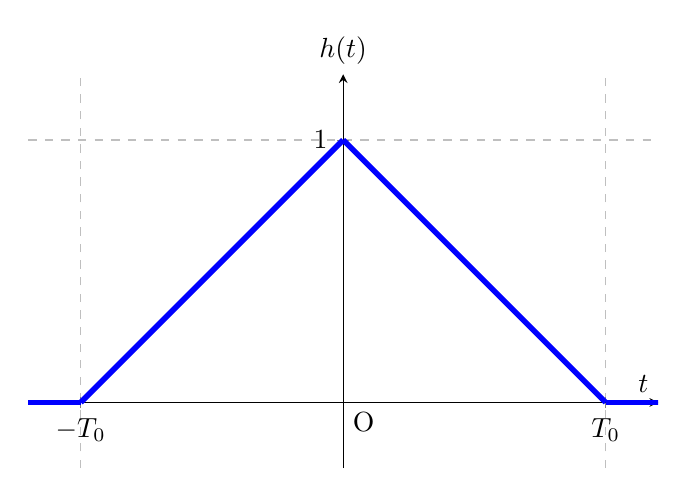
\begin{tikzpicture}
            \begin{axis}[
                axis lines = middle,
                xlabel = {$t$},
                ylabel = {$h(t)$},
                ylabel style={at={(rel axis cs:0.5, 1)}, anchor=south},
                xmin = -1.2, xmax = 1.2,
                ymin = -0.2, ymax = 1.2,
                xtick = {-1, 0, 1},
                xticklabels = {$-T_0$, $ $, $T_0$},
                ytick distance = 1,
                grid = major,
                grid style = dashed,
                scale only axis,
                width = 8cm,
                height = 5cm,
                axis equal,
            ]
            \addplot[domain=-1.2:-1, samples=100, smooth, line width=2pt, blue] {0};
            \addplot[domain=-1:0, samples=100, smooth, line width=2pt, blue] {x + 1};
            \addplot[domain=0:1, samples=100, smooth, line width=2pt, blue] {-x + 1};
            \addplot[domain=1:1.2, samples=100, smooth, line width=2pt, blue] {0};
            \node at (axis cs:0, 0) [anchor=north west] {O};
            \end{axis}
        \end{tikzpicture}
        \caption{三角信号 $h(t)$}
        \label{fig:triangular-rectangular-1}
    \end{figure}
    则其傅里叶变换为
    \begin{align*}
        H(\mathi\omega) = T_0\cdot \sa^2\left(\frac{\omega T_0}{2}\right).
    \end{align*}
\end{property}

\begin{proof}
    三角脉冲可以表示为两个矩形脉冲的卷积。记 $g(t)$ 为 $[-T_0/2, T_0/2]$ 上的矩形脉冲信号,
    脉宽 $\tau = T_0$,脉高 $E = \sqrt{1/T_0}$,如图 \ref{fig:triangular-rectangular-2} 所示。
    \begin{figure}[H]
        \centering
        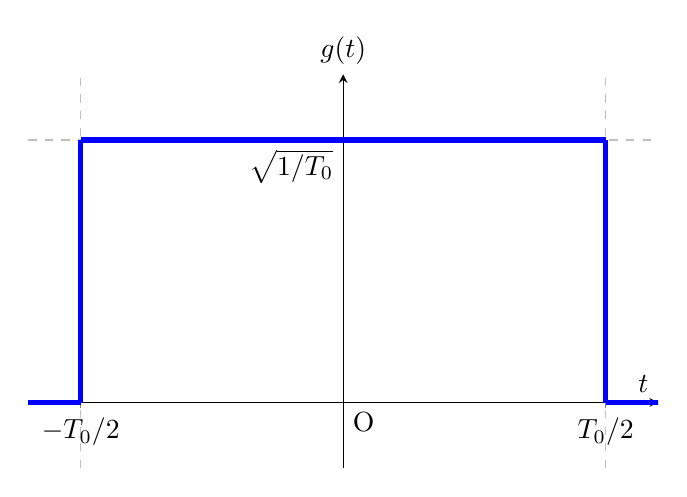
\begin{tikzpicture}
            \begin{axis}[
                axis lines = middle,
                xlabel = {$t$},
                ylabel = {$g(t)$},
                ylabel style={at={(rel axis cs:0.5, 1)}, anchor=south},
                xmin = -1.2, xmax = 1.2,
                ymin = -0.2, ymax = 1.2,
                xtick = {-1, 0, 1},
                xticklabels = {$-T_0/2$, $ $, $T_0/2$},
                ytick = {0, 1},
                yticklabels = {$ $, $ $},
                grid = major,
                grid style = dashed,
                scale only axis,
                width = 8cm,
                height = 5cm,
                axis equal,
            ]
            \addplot[domain=-1.2:-1, samples=100, smooth, line width=2pt, blue] {0};
            \addplot[smooth, line width=2pt, blue] coordinates {(-1, 0) (-1, 1)};
            \addplot[domain=-1:0, samples=100, smooth, line width=2pt, blue] {1};
            \addplot[domain=0:1, samples=100, smooth, line width=2pt, blue] {1};
            \addplot[smooth, line width=2pt, blue] coordinates {(1, 1) (1, 0)};
            \addplot[domain=1:1.2, samples=100, smooth, line width=2pt, blue] {0};
            \node at (axis cs:0, 0) [anchor=north west] {O};
            \node at (axis cs:0, 1) [anchor=north east] {$\sqrt{1/T_0}$};
            \end{axis}
        \end{tikzpicture}
        \caption{矩形脉冲信号 $g(t)$}
        \label{fig:triangular-rectangular-2}
    \end{figure}
    因此,$h(t) = g(t) * g(t)$。由卷积定理知
    \begin{align*}
        H(\mathi\omega) & = G(\mathi\omega) \cdot G(\mathi\omega) \\
        & = \left(E\tau\sa\left(\frac{\omega\tau}{2}\right)\right)^2 \\
        & = T_0\cdot \sa^2\left(\frac{\omega T_0}{2}\right).
    \end{align*}
\end{proof}

\begin{definition}[欠采样]
    如果采样时不满足采样定理的要求,则一定会在 $x(t)$ 的频谱周期延拓时,
    出现\bd{频谱混叠}的现象,这种现象称为\bd{欠采样}。
    从用样本代替信号的角度出发,出现欠采样的情况是工程应用中不希望的。

    \begin{enumerate}
        \item 频谱混叠的情况下时域信号变了,但采样点处取值不变。
        
            此时,即使通过理想内插也得不到原信号。
            但是无论怎样,恢复所得的信号 $x(t)$ 与原信号 $x(t)$ 在采样点上
            将具有相同的值,即 $x_r(nT_s) = x(nT_s)$。

            例如对信号 $x(t) = \cos\omega_0 t$ 进行欠采样。$x(t)$ 的频谱 $X(\mathi\omega)$ 为
            \begin{align*}
                X(\mathi\omega) & = \mathcal{F}[x(t)] \\
                & = \mathcal{F}[\cos\omega_0 t] \\
                & = \mathcal{F}\left[\frac{\mathe^{\mathi\omega_0 t} + \mathe^{-\mathi\omega_0 t}}{2}\right] \\
                & = \pi(\delta(\omega - \omega_0) + \delta(\omega + \omega_0)).
            \end{align*}
            当 $\omega_0 < \omega_s < 2\omega_0$ 时,产生频谱混叠。此时,
            如图 \ref{fig:undersampling} 所示,
            恢复的信号为
            \begin{align*}
                x_r(t) = \cos(\omega_s - \omega_0) t.
            \end{align*}
            \begin{figure}[H]
                \centering
                \includegraphics[width=0.6\textwidth]{chap2/img/undersampling.png}
                \caption{欠采样}
                \label{fig:undersampling}
            \end{figure}
            当 $t = nT_s$ 时,有
            \begin{align*}
                x_r(nT_s) & = \cos(\omega_s - \omega_0) nT_s \\
                & = \cos(\omega_s n T_s - \omega_0nT_s) \\
                & = \cos(2n\pi - \omega_0 n T_s) \\
                & = \cos\omega_0 n T_s \\
                & = x(nT_s).
            \end{align*}
        \item 工程应用时,如果采样频率 $\omega_s = 2\omega_M$,则
            不足以从样本中恢复原信号。

            例如对信号 $x(t) = \cos(\omega_0 t + \varphi)$ 在 $\omega_s = 2\pi/T_s = 2\omega_0$ 条件下
            进行采样,则
            \begin{align*}
                x(nT) & = \cos(\omega_0 nT_s + \varphi) \\
                & = \cos\varphi\cos(\omega_0 nT_s) - \sin\varphi\sin(\omega_0 nT_s) \\
                & = \cos\varphi\cos n\omega_0 T_s.
            \end{align*}
            这与对 $x_1(t) = \cos\varphi\cos\omega_0 t$ 进行采样得到的结果相同,
            所以,无法判断恢复后的信号是 $x(t)$ 还是 $x_1(t)$。        
        \item 对信号进行二次采样,可以看做是第一次采样的到了一个离散信号,再对这个离散信号进行采样。
            \begin{figure}[H]
                \centering
                \includegraphics[width=0.3\textwidth]{chap2/img/resampling.png}
                \caption{二次采样}
                \label{fig:resampling.png}
            \end{figure}
            如图 \ref{fig:resampling.png} 所示,$x(n)$ 中黑色和红色的信号表示第一次采样后的信号,
            再使用 $p(n)$ 作为采样信号,再次采样后得到的信号为 $x_p(n)$,即为红色信号。
    \end{enumerate}
\end{definition}


\begin{exercise}
    试证明:当对信号 $x(t) = \cos(\omega_0 t + \varphi)$ 欠采样时,
    恢复的信号不仅频率降低,而且相位相反。其中,$\omega_0 < \omega_s < 2\omega_0$,
    且理想低通滤波器的截止频率 $\omega_c \in (\omega_s - \omega_0, \omega_0)$。
\end{exercise}

\begin{proof}
    展开 $x(t)$ 可得
    \begin{align*}
        x(t) = \cos(\omega_0 t + \varphi) = \cos\varphi\cos\omega_0 t- \sin\varphi \sin\omega_0 t.
    \end{align*}
    因此,
    \begin{align*}
        X(\mathi\omega) & = \mathcal{F}[x(t)] \\
        & = \cos\varphi\cdot \pi[\delta(\omega - \omega_0) + \delta(\omega + \omega_0)]
            + \sin\varphi\cdot \mathi\pi[\delta(\omega - \omega_0) - \delta(\omega + \omega_0)] \\
        & = (\cos\varphi + \mathi\sin\varphi)\pi\delta(\omega - \omega_0)
            + (\cos\varphi - \mathi\sin\varphi)\pi\delta(\omega + \omega_0).
    \end{align*}
    类似 \ref{fig:undersampling},当 $\omega_s < 2\omega_0$ 时,产生频谱混叠。此时,
    \begin{align*}
        X_r(\mathi\omega) = (\cos\varphi - \mathi\sin\varphi)\pi\delta(\omega - \omega_0 + \omega_s)
            + (\cos\varphi + \mathi\sin\varphi)\pi\delta(\omega + \omega_0 - \omega_s).
    \end{align*}
    因此
    \begin{align*}
        x_r(t) = \mathcal{F}^{-1}[X_r(\mathi\omega)] & = \cos\varphi\cos((\omega_0 - \omega_s)t)
            - \sin\varphi\sin((\omega_0 - \omega_s)t) \\
        & = \cos((\omega_0 - \omega_s)t + \varphi) \\
        & = \cos((\omega_s - \omega_0)t - \varphi).
    \end{align*}
    由于 $\omega_s < 2\omega_0$,故 $\omega_s - \omega_0 < \omega_0$,即 $\omega_s - \omega_0$ 为正频率。
    因此,恢复的信号不仅频率降低,而且相位相反。命题得证。
\end{proof}

\subsubsection{频域采样}

采样的本质是把连续变量的函数离散化。因此,在频域上也可以对连续的频谱进行采样,这一过程与时域采样是完全对偶的。

\begin{definition}[频域采样]
    频域采样的数学模型如图 \ref{fig:sampling-freq-math-model} 所示,
    其中 $p(t)$ 是采样脉冲,$P(\mathi \omega)$ 是 $p(t)$ 的傅里叶变换。
    \begin{figure}[H]
        \centering
        \begin{tikzpicture}
            \draw (0,0) circle (0.25);
        
            \draw (-0.177,-0.177) -- (0.177,0.177);
            \draw (0.177,-0.177) -- (-0.177,0.177);
        
            \draw[->] (-1.5,0) -- (-0.5,0);
            \draw[->] (0.5,0) -- (1.5,0);
            \draw[->] (0,-1.5) -- (0,-0.5);
        
            \node at (-2,0) {$X(\mathi\omega)$};
            \node at (2,0) {$X_p(\mathi\omega)$};
            \node at (0,-2) {$P(\mathi\omega)$};
        \end{tikzpicture}
        \caption{频域采样的数学模型}
        \label{fig:sampling-freq-math-model}
    \end{figure}

    \begin{itemize}
        \item 在频域上,$X_p(\mathi \omega) = X(\mathi \omega) P(\mathi \omega)$。
        \item 在时域上,$x_p(t) = x(t) * p(t)$。
    \end{itemize}
    当采样为\bd{冲激串采样}(\bd{理想采样})时,
    \begin{align*}
        P(\mathi\omega) & = \sum_{n = -\infty}^{+\infty}\delta(\omega - n\omega_s), \\
        X_p(\mathi\omega) & = X(\mathi\omega)P(\mathi\omega) = \sum_{n = -\infty}^{+\infty}X(n\omega_s)\delta(\omega - n\omega_0),
    \end{align*}
    其中 $\omega_s$ 为采样间隔。
\end{definition}

\begin{example}
    如图 \ref{fig:impulse-sampling-freq} 所示,
    为利用冲激串进行采样的信号 $X(\mathi\omega)$ 与 $X_p(\mathi\omega)$,
    其中采样间隔 $\omega_s = \omega_0$。
    \begin{figure}[H]
        \centering
        \includegraphics[width=0.45\textwidth]{chap2/img/impulse-sampling-freq.png}
        \caption{冲激串采样的信号 $X(\mathi\omega)$ 与 $X_p(\mathi\omega)$}
        \label{fig:impulse-sampling-freq}
    \end{figure}
\end{example}

\begin{property}
    冲激串信号 $P(\mathi\omega)$ 的逆傅里叶变换 $\mathcal{F}^{-1}[P(\mathi\omega)] = p(t)$ 为
    \begin{align*}
        p(t) = \frac{1}{\omega_s}\sum_{n = -\infty}^{+\infty}\delta(t - \frac{2\pi}{\omega_s}n).
    \end{align*}
\end{property}

\begin{proof}
    证明略。过程类似于 \ref{property:impulse-sampling-frequency-1} 的证明。
\end{proof}

\begin{property}
    冲激串采样后的信号 $X_p(\mathi\omega)$ 的逆傅里叶变换 $\mathcal{F}^{-1}[X_p(\mathi\omega)] = x_p(t)$ 为
    \begin{align*}
        x_p(t) = \frac{1}{\omega_s}\sum_{n = -\infty}^{+\infty}x(t - \frac{2\pi}{\omega_s}n).
    \end{align*}
\end{property}

\begin{proof}
    证明略。过程类似于 \ref{property:impulse-sampling-frequency-2} 的证明。
\end{proof}

\begin{remark}
    由此可见,在频域对连续频谱进行理想采样,
    就相当于在时域将信号\bd{以 $2\pi/\omega_s$ 为周期进行延拓}。
\end{remark}

\begin{definition}[时限内插]
    在频域上,从频域的样本重建连续频谱的过程称为\bd{时限内插}。
    时限内插是以矩形窗函数的频谱作为内插函数实现的。

    矩形窗函数 $w(t) = \begin{cases}
        \omega_s, & |t| \le \pi/\omega_s, \\
        0, & |t| > \pi/\omega_s.
    \end{cases}$ 的频谱为
    \begin{align*}
        W(\mathi\omega) = 2\pi \sa{\left(\frac{\pi\omega}{\omega_s}\right)}.
    \end{align*}

    \bd{理想时限内插}重建得到的信号 $X(\mathi\omega)$ 为
    \begin{align*}
        X(\mathi\omega) & = \frac{1}{2\pi}X_p(\mathi\omega) * W(\mathi\omega) \\
        & = \frac{1}{2\pi} \sum_{n = -\infty}^{+\infty}X(n\omega_s)\delta(\omega - n\omega_s) * 2\pi\sa{\left(\frac{\pi\omega}{\omega_s}\right)} \\
        & = \sum_{n = -\infty}^{+\infty}X(n\omega_s)\sa{\left(\frac{\pi(\omega - n\omega_s)}{\omega_s}\right)}.
    \end{align*}
\end{definition}

\begin{note}
    带限和时限\bd{没有必然的逻辑联系}。请注意时域采样定理应用条件中的{带限要求},
    频域采样定理应用条件中的\bd{时限要求}。因此,对带限信号在频域采样时,如果时域没有说明是时限,
    则不能保证频谱的样本可以恢复原信号。
\end{note}

